\documentclass[12pt]{article}

\usepackage{amsthm}
\usepackage{amsmath}
\usepackage{amsfonts}
\usepackage{algorithm}
\usepackage{algpseudocode}
\usepackage{mathrsfs}
\usepackage{array}
\usepackage{amssymb}
\usepackage{units}
\usepackage{graphicx}
\usepackage{tikz-cd}
\usepackage{nicefrac}
\usepackage{hyperref}
\usepackage{bbm}
\usepackage{color}
\usepackage{tensor}
\usepackage{tipa}
\usepackage{bussproofs}
\usepackage{ stmaryrd }
\usepackage{ textcomp }
\usepackage{leftidx}
\usepackage{afterpage}
\usepackage{varwidth}
\usepackage{tasks}
\usepackage{ cmll }
\usepackage{quiver}
\usepackage{adjustbox}
\usepackage{kbordermatrix}

\newcommand\blankpage{
	\null
	\thispagestyle{empty}
	\addtocounter{page}{-1}
	\newpage
}

\graphicspath{ {images/} }

\theoremstyle{plain}
\newtheorem{thm}{Theorem}[subsection] % reset theorem numbering for each chapter
\newtheorem{proposition}[thm]{Proposition}
\newtheorem{lemma}[thm]{Lemma}
\newtheorem{fact}[thm]{Fact}
\newtheorem{cor}[thm]{Corollary}

\theoremstyle{definition}
\newtheorem{defn}[thm]{Definition} % definition numbers are dependent on theorem numbers
\newtheorem{exmp}[thm]{Example} % same for example numbers
\newtheorem{notation}[thm]{Notation}
\newtheorem{remark}[thm]{Remark}
\newtheorem{condition}[thm]{Condition}
\newtheorem{question}[thm]{Question}
\newtheorem{construction}[thm]{Construction}
\newtheorem{exercise}[thm]{Exercise}
\newtheorem{example}[thm]{Example}
\newtheorem{aside}[thm]{Aside}

\def\doubleunderline#1{\underline{\underline{#1}}}
\newcommand{\bb}[1]{\mathbb{#1}}
\newcommand{\scr}[1]{\mathscr{#1}}
\newcommand{\call}[1]{\mathcal{#1}}
\newcommand{\psheaf}{\text{\underline{Set}}^{\scr{C}^{\text{op}}}}
\newcommand{\und}[1]{\underline{\hspace{#1 cm}}}
\newcommand{\adj}[1]{\text{\textopencorner}{#1}\text{\textcorner}}
\newcommand{\comment}[1]{}
\newcommand{\lto}{\longrightarrow}
\newcommand{\rone}{(\operatorname{R}\bold{1})}
\newcommand{\lone}{(\operatorname{L}\bold{1})}
\newcommand{\rimp}{(\operatorname{R} \multimap)}
\newcommand{\limp}{(\operatorname{L} \multimap)}
\newcommand{\rtensor}{(\operatorname{R}\otimes)}
\newcommand{\ltensor}{(\operatorname{L}\otimes)}
\newcommand{\rtrue}{(\operatorname{R}\top)}
\newcommand{\rwith}{(\operatorname{R}\&)}
\newcommand{\lwithleft}{(\operatorname{L}\&)_{\operatorname{left}}}
\newcommand{\lwithright}{(\operatorname{L}\&)_{\operatorname{right}}}
\newcommand{\rplusleft}{(\operatorname{R}\oplus)_{\operatorname{left}}}
\newcommand{\rplusright}{(\operatorname{R}\oplus)_{\operatorname{right}}}
\newcommand{\lplus}{(\operatorname{L}\oplus)}
\newcommand{\prom}{(\operatorname{prom})}
\newcommand{\ctr}{\operatorname{ctr}}
\newcommand{\der}{(\operatorname{der})}
\newcommand{\weak}{\operatorname{weak}}
\newcommand{\exi}{(\operatorname{exists})}
\newcommand{\fa}{(\operatorname{for\text{ }all})}
\newcommand{\ex}{(\operatorname{ex})}
\newcommand{\cut}{\operatorname{cut}}
\newcommand{\ax}{\operatorname{ax}}
\newcommand{\negation}{\sim}
\newcommand{\true}{\top}
\newcommand{\false}{\bot}
\newcommand{\LM}{\operatorname{LM}}
\newcommand{\LT}{\operatorname{LT}}
\def\l{\,|\,}
\newcommand{\ediv}[2]{\operatorname{div}(#1,#2)}
\newcommand{\edives}[2]{\operatorname{div}_{es}(#1,#2)}
\newcommand{\multideg}{\operatorname{multideg}}
\newcommand{\pax}{\operatorname{pax}}
\DeclareRobustCommand{\diamondtimes}{%
	\mathbin{\text{\rotatebox[origin=c]{45}{$\boxplus$}}}%
}
\newcommand{\tagarray}{\mbox{}\refstepcounter{equation}$(\theequation)$}
\newcommand{\startproof}[1]{
	\AxiomC{#1}
	\noLine
	\UnaryInfC{$\vdots$}
}
\newenvironment{scprooftree}[1]%
{\gdef\scalefactor{#1}\begin{center}\proofSkipAmount \leavevmode}%
	{\scalebox{\scalefactor}{\DisplayProof}\proofSkipAmount \end{center} }

\usepackage[margin=2.5cm]{geometry}


\title{Elimination and cut-elimination (exponentials)}
\author{Will Troiani}
\date{\today}

\begin{document}

\maketitle
\tableofcontents

\section{Background}
We recall the definitions of \emph{unoriented atoms}.

\begin{defn}
\label{def:atomic_atoms}
There is an infinite set of \textbf{unoriented atoms} $X,Y,Z,\ldots$ and an \textbf{oriented atom} (or \textbf{atomic proposition}) is a pair $(X,+)$ or $(X,-)$ where $X$ is an unoriented atom. Let $\call{A}$ denote the set of oriented atoms.
\end{defn}

For $x \in \{ +, - \}$ we write $\overline{x}$ for the negation, so $\overline{+} = -, \overline{-} = +$.

\begin{defn}
The set of \textbf{pre-formulas} is defined as follows:
\begin{itemize}
	\item Any atomic proposition is a preformula.
	\item If $A,B$ are pre-formulas then so are $A \otimes B, A \parr B$.
	\item If $A$ is a pre-formula then so are $\neg A, ! A, ? A$.
\end{itemize}
The set of \textbf{multiplicative exponential linear logic formulas (MELL formulas)} is the quotient of the set of pre-formulas by the equivalence relation generated, for arbitrary formulas $A, B$ and unoriented atom $X$, by
\begin{align*}
\neg(A \otimes B) &= \neg B \parr \neg A,\quad \neg(A \parr B) = \neg B \otimes A,\quad \neg(X, x) = (X, \overline{x})\\
\neg !A &= ? \neg A,\quad \neg ?A = !\neg A
\end{align*}
\end{defn}

Recall that in the multiplicative case, the set of words $\call{A}^\ast$ over $\call{A}$ forms a monoid under the operation of concatination. This monoidal structure extends to maps reflecting the connectives $\otimes, \parr, \neg$, for instance if $c: \call{A}^\ast \times \call{A}^\ast \lto \call{A}^\ast$ denotes concatination, and $\otimes: \call{F} \times \call{F} \lto \call{F}$ is the map sending a pair of formulas $A,B$ to the formula $A \otimes B$ then the following diagram commutes for some unique map $a: \call{F} \lto \call{A}^\ast$.
\begin{equation}
\begin{tikzcd}
\call{F} \times \call{F}\arrow[r,"{a \times a}"]\arrow[d,swap,"{\otimes}"] & \call{A}^\ast \times \call{A}^\ast\arrow[d,"{c}"]\\
\call{F}\arrow[r,"{a}"] & \call{A}^\ast
\end{tikzcd}
\end{equation}
See \cite[Definition 3.5, 3.6]{MT} for the full list of commutative diagrams. This map $a$ induces the \textbf{sequence of oriented atoms} of a formula $A$.
\begin{equation}
a(A) = (X_1, x_1), \ldots, (X_n, x_n)
\end{equation}
The \textbf{set of unoriented atoms} of $A$ is then the disjoint union
\begin{equation}
U_A = \{ X_1 \} \coprod \ldots \coprod \{ X_n \}
\end{equation}
We use this notation in the following Definition.
\begin{defn}\label{def:unoriented_atoms}
Let $A$ be a multiplicative exponential linear logic formula. The \textbf{set of unoriented atoms} $U_A$ of $A$ is defined by induction on the structure of $A$ as follows.
\begin{itemize}
	\item If $A = A_1 \otimes A_2$ or $A_1 \parr A_2$ then $U_A := U_{A_1} \coprod U_{A_2}$.
	\item If $A = \neg A'$ then $U_{A} := U_{A'}$.
	\item If $A = ?A'$ or $A = !A'$ then $U_A := \bb{N} \times U_{A'}$.
\end{itemize}
\end{defn}

\begin{example}
Let $(X_1, +), (X_2, -)$ be atoms and set $A = !(X_1, +) \otimes !(X_2, -)$ and $B = !\big((X_1, +) \otimes (X_2, -)\big)$. Then
\begin{align*}
U_A &= \big(\bb{N} \times \{ X_1 \}\big) \coprod \big(\bb{N} \times \{ X_2 \}\big)\\
U_B &= \bb{N} \times \{ X_1, X_2 \}
\end{align*}
\end{example}
Now we extend the definition of a multiplicative proof structure to a multiplicative exponential proof structure. For clarity, we rewrite the entire definition, including that of the multiplicative fragment which appears in \cite[Definition 3.9]{MT}.
\begin{defn}
\label{def:proof_structure}
A \textbf{proof structure} is a directed multigraph with edges labelled by formulas and with vertices labelled by $\ax, \cut, \otimes, \parr, !, ?, \operatorname{ctr}, \operatorname{wk}, \operatorname{pax}$ or $\operatorname{c}$. The incoming edges of a vertex are called its \textbf{premises}, the outgoing edges are its \textbf{conclusions}. Proof structures are required to adhere to the following conditions:
\begin{itemize}
	\item Each vertex labelled $\ax$ has exactly two conclusions and no premise, the conclusions are labelled $A$ and $\neg A$ for some $A$. We call this an \textbf{axiom link}.
	\item Each vertex labelled $\cut$ has exactly two premises and no conclusion, where the premises are labelled $A$ and $\neg A$ for some $A$. We call this a \textbf{cut link}.
	\item Each vertex labelled $\otimes$ has exactly two premises and one conclusion. The premises are ordered, the smallest one is called the \textbf{left} premise of the vertex, the biggest one is called the \textbf{right} premise. The left premise is labelled $A$, the right premise is labelled $B$ and the conclusions is labelled $A \otimes B$, for some $A, B$. We call this a \textbf{tensor link}.
	\item Each vertex labelled $\parr$ has exactly two ordered premises and one conclusion. The left premise is labelled $A$, the right premise is labelled $B$ and the conclusion is labelled $A \parr B$, for some $A, B$. We call this a \textbf{par link}.
	\item Each vertex labelled $\operatorname{ctr}$ has exactly two premises and one conclusion. The left premise, the right premise, and the conclusion are all labelled $? A$ for some $A$. We call this a \textbf{contraction link}.
	\item Each vertex labelled $\operatorname{pax}$ has exactly one premise and one conclusion. The premise and conclusion are both labelled $?A$ for some formula $A$. We call this a \textbf{pax link}. Pax links are only allowed to exist when they are associated with promotion links, see the following clause.
	\item Each vertex labelled $!$ has exactly one premise and one conclusion. The premise is labelled $A$ for some $A$, and the conclusion by $! A$. We call this a \textbf{promotion link}. Each promotion link must come equipt with a selection of the pax links so that everything lying above these pax links and the promotion link itself form a proof structure, when these pax and promotion links are replaced with conclusion links.
	\item Each vertex labelled $\operatorname{weak}$ has no premises and one conclusion. The conclusion is labelled $?A$ for some $A$. We call this a \textbf{weakening link}.
	\item Each vertex labelled $?$ has exactly one premise and one conclusion. The premise is labelled $A$ for some $A$, and the conclusion by $? A$. We call this a \textbf{dereliction link}.
	\item Each vertex labelled $\operatorname{c}$ has exactly one premise and no conclusion. Such a premise of a vertex labelled $c$ is called a \textbf{conclusion} of the proof structure.
\end{itemize}
\end{defn}
\begin{remark}
In Definition \ref{def:proof_structure} the choices of vertices in the clauses pertaining to the weakening and promotion links must be explicitly given, and are understood to be associated to their respective links. This is denoted graphically by putting these links inside boxes, everything ``inside" the box is an element of the subset corresponding to the link.
\end{remark}
\begin{defn}
Let $A$ be an occurrence of a formula inside a proof structure $\pi$. The \textbf{depth} of $A$ is the number of times it appears in the subset of $\pi$ corresponding to a promotion link.
\end{defn}

In the multiplicative case \cite{MT} we used the atomic propositions of a formula to define the \emph{polynomial ring} \cite[Definition 3.14]{MT} of a formula, and ultimately the \emph{coordinate ring} \cite[Definition 3.21]{MT} of a proof structure.

In the case of MELL, the definition is more complicated, because we need to take the concept of depth into account. Thus we have two notions, the \emph{unoriented atoms of a formula}, just defined \ref{def:unoriented_atoms}, and the unoriented atoms \emph{with respect to the formula's depth inside a proof structure}, which we define now.

\begin{defn}
Let $\pi$ be a proof structure and $A$ a depth $d$ occurrence of a formula in $\pi$.

The \textbf{unoriented atoms} of $A$ in $\pi$, $\operatorname{Dep}U_A$ is
\begin{equation}
\operatorname{Dep}U_A := \bb{N}^d \times U_A
\end{equation}
\end{defn}

\begin{remark}
Every element of $\operatorname{Dep}U_A$ is of the form
\begin{equation}
(\underline{j}, X_i)
\end{equation}
where $\underline{j}$ is a finite sequence (possibly of length 0) of natural numbers, and $X_i$ is an unoriented atom of some set $U_B$ for a multiplicative formula $B$.
\end{remark}

\begin{defn}
Let $\pi$ be a proof structure and $A$ a depth $d$ occurrence of a formula inside $\pi$. The \textbf{polynomial ring} $P_{A}$ associated to $A$ is the free commutative $k$-algebra on the set $\operatorname{Dep}U_{A}$ of unoriented atoms of $A$ in $\pi$.
\end{defn}

\begin{defn}
The \textbf{set of unoriented atoms with respect to depth} of a proof structure $\pi$ is the disjoint union $\operatorname{Dep}U_\pi = \coprod_{e \in E}\operatorname{Dep}U_{A_e}$ where $E$ is the set of edges in $\pi$ and for each $e \in E$ we write $\operatorname{Dep}U_{A_e}$ for the set of unoriented atoms of the formula $A_e$ in $\pi$ where $A_e$ is labelling $e$.
\end{defn}

\begin{defn}
The \textbf{polynomial ring of a proof structure} $\pi$, $P_\pi$, is the free commutative $k$-algebra on the set $\operatorname{Dep}U_\pi$ of unoriented atoms of $\pi$.
\end{defn}

The ideal generated by a set $S$ is denoted $\langle S \rangle$. For each type of link $l$ we define the \textbf{generating set} $G_l$ and \textbf{link ideal} $I_l = \langle G_l \rangle$ in the polynomial ring generated by the set of unoriented atoms of formulas labelling edges incident at the link.

\begin{defn}
If $l$ is one of the links
% https://q.uiver.app/?q=WzAsNyxbMSwwLCJcXGF4Il0sWzAsMSwiXFx2ZG90cyJdLFsyLDEsIlxcdmRvdHMiXSxbNCwwXSxbNCwxLCJcXGN1dCJdLFszLDAsIlxcdmRvdHMiXSxbNSwwLCJcXHZkb3RzIl0sWzAsMSwiXFxuZWcgQSIsMix7ImN1cnZlIjoyfV0sWzAsMiwiQSIsMCx7ImN1cnZlIjotMn1dLFs1LDQsIkEiLDIseyJjdXJ2ZSI6Mn1dLFs2LDQsIlxcbmVnIEEiLDAseyJjdXJ2ZSI6LTJ9XV0=
\[\begin{tikzcd}
	& \ax && \vdots & {} & \vdots \\
	\vdots && \vdots && \cut
	\arrow["{\neg A}"', curve={height=12pt}, from=1-2, to=2-1]
	\arrow["A", curve={height=-12pt}, from=1-2, to=2-3]
	\arrow["A"', curve={height=12pt}, from=1-4, to=2-5]
	\arrow["{\neg A}", curve={height=-12pt}, from=1-6, to=2-5]
\end{tikzcd}\]
then there is one inclusion map per displayed occurrence of a formula
\begin{align*}
\iota_{A}: \operatorname{Dep}U_A &\lto \operatorname{Dep}U_\pi\\
\iota_{\neg A}: \operatorname{Dep}U_{\neg A} &\lto \operatorname{Dep}U_{\pi}
\end{align*}
For each $\mathbf{X} \in \operatorname{Dep}U_A$, we use the fact that $\operatorname{Dep}U_A = \operatorname{Dep}U_{\neg A}$ to define the polynomial
\begin{equation}
\iota_A(\textbf{X}) - \iota_{\neg A}(\textbf{X}) \in P_{\pi}
\end{equation}

The set $G_l$ consists of all such polynomials, and no further polynomials.
\end{defn}

\begin{defn}
If $l$ is one of the links
% https://q.uiver.app/?q=WzAsOCxbMSwxLCJcXHBhcnIiXSxbMCwwLCJcXHZkb3RzIl0sWzIsMCwiXFx2ZG90cyJdLFsxLDIsIlxcdmRvdHMiXSxbMywwLCJcXHZkb3RzIl0sWzUsMCwiXFx2ZG90cyJdLFs0LDEsIlxcb3RpbWVzIl0sWzQsMiwiXFx2ZG90cyJdLFsxLDAsIkEiLDIseyJjdXJ2ZSI6Mn1dLFsyLDAsIkIiLDAseyJjdXJ2ZSI6LTJ9XSxbMCwzLCJBIFxccGFyciBCIl0sWzQsNiwiQSIsMix7ImN1cnZlIjoyfV0sWzUsNiwiQiIsMCx7ImN1cnZlIjotMn1dLFs2LDcsIkEgXFxvdGltZXMgQiJdXQ==
\[\begin{tikzcd}
	\vdots && \vdots & \vdots && \vdots \\
	& \parr &&& \otimes \\
	& \vdots &&& \vdots
	\arrow["A"', curve={height=12pt}, from=1-1, to=2-2]
	\arrow["B", curve={height=-12pt}, from=1-3, to=2-2]
	\arrow["{A \parr B}", from=2-2, to=3-2]
	\arrow["A"', curve={height=12pt}, from=1-4, to=2-5]
	\arrow["B", curve={height=-12pt}, from=1-6, to=2-5]
	\arrow["{A \otimes B}", from=2-5, to=3-5]
\end{tikzcd}\]
For each displayed edge there is an inclusion 
\begin{align*}
\iota_A: \operatorname{Dep}U_A &\lto \operatorname{Dep}U_{\pi}\\
\iota_B: \operatorname{Dep}U_B &\lto \operatorname{Dep}U_{\pi}\\
\iota_{A \boxtimes B}: \operatorname{Dep}U_{A \boxtimes B} &\lto \operatorname{Dep}U_{\pi}
\end{align*}
where $\boxtimes$ is either $\otimes$ or $\parr$. For each $\textbf{X} \in \operatorname{Dep}U_A$ there is a corresponding $\textbf{X}' \in \operatorname{Dep}U_{A \boxtimes B}$. Similarly, for each $\textbf{Y} \in \operatorname{Dep}U_{B}$ there is a corresponding $\textbf{Y}' \in \operatorname{Dep}U_{A \boxtimes B}$

For each $\textbf{X} \in \operatorname{Dep}U_{A}$ and each $\textbf{Y} \in \operatorname{Dep}U_B$, the polynomials
\begin{equation}
\iota_A(\textbf{X}) - \iota_{A \boxtimes B}(\textbf{X}'),\qquad \iota_B(\textbf{Y}) - \iota_{A \boxtimes B}(\textbf{Y}')
\end{equation}
are elements of $G_l$.
\end{defn}

\begin{defn}
If $l$ is a dereliction link
% https://q.uiver.app/?q=WzAsMyxbMCwwLCJcXHZkb3RzIl0sWzAsMSwiPyJdLFswLDIsIlxcdmRvdHMiXSxbMCwxLCJBIl0sWzEsMiwiP0EiXV0=
\[\begin{tikzcd}
	\vdots \\
	{?} \\
	\vdots
	\arrow["A", from=1-1, to=2-1]
	\arrow["{?A}", from=2-1, to=3-1]
\end{tikzcd}\]
There exist inclusion maps
\begin{align*}
\iota_A: \operatorname{Dep}U_{A} &\lto \operatorname{Dep}U_{\pi}\\
\iota_{?A}: \operatorname{Dep}U_{?A} &\lto \operatorname{Dep}U_{\pi}
\end{align*}
We use the fact that $\operatorname{Dep}U_{?A} = \bb{N} \times \operatorname{Dep}U_A$ to define the polynomials
\begin{equation}
\iota_A(\textbf{X}) - \iota_{?A}\big((j, \textbf{X})\big)
\end{equation}
ranging over all $j \geq 0$. These are the polynomials of $G_l$.
\end{defn}

\begin{defn}
If $l$ is a pax link
% https://q.uiver.app/?q=WzAsNSxbMSwwLCJcXHZkb3RzIl0sWzEsMSwiXFxwYXgiXSxbMSwyLCJcXHZkb3RzIl0sWzIsMSwiXFxkb3RzIl0sWzAsMSwiXFxkb3RzIl0sWzEsMywiIiwwLHsic3R5bGUiOnsiaGVhZCI6eyJuYW1lIjoibm9uZSJ9fX1dLFs0LDEsIiIsMCx7InN0eWxlIjp7ImhlYWQiOnsibmFtZSI6Im5vbmUifX19XSxbMCwxLCI/QSJdLFsxLDIsIj9BIl1d
\[\begin{tikzcd}
	& \vdots \\
	\dots & \pax & \dots \\
	& \vdots
	\arrow[no head, from=2-2, to=2-3]
	\arrow[no head, from=2-1, to=2-2]
	\arrow["{?A}", from=1-2, to=2-2]
	\arrow["{?A}", from=2-2, to=3-2]
\end{tikzcd}\]
Let the premise be labelled $?A_p$ and the conclusion $?A_c$. We have
\begin{equation}
\operatorname{Dep}U_{?A_p} = \bb{N}^2 \times \operatorname{Dep}U_{A},\qquad \operatorname{Dep}U_{?A_c} = \bb{N} \times \operatorname{Dep}U_{A_p}
\end{equation}
There exist inclusion maps
\begin{align*}
\iota_{?A_p}: \operatorname{Dep}U_{?A_p} &\lto \operatorname{Dep}U_\pi\\
\iota_{?A_c}: \operatorname{Dep}U_{?A_c} &\lto \operatorname{Dep}U_{\pi}
\end{align*}
The polynomials
\begin{equation}
(j_0, j_1, \textbf{X}) - (j_1, \textbf{X})
\end{equation}
for $\textbf{X} \in \operatorname{Dep}U_A$ are the polynomials of $G_l$.
\end{defn}

\begin{defn}
If $l$ is a promotion link
% https://q.uiver.app/?q=WzAsNSxbMSwwLCJcXHZkb3RzIl0sWzEsMSwiISJdLFsxLDIsIlxcdmRvdHMiXSxbMiwxLCJcXGRvdHMiXSxbMCwxLCJcXGRvdHMiXSxbMSwzLCIiLDAseyJzdHlsZSI6eyJoZWFkIjp7Im5hbWUiOiJub25lIn19fV0sWzQsMSwiIiwwLHsic3R5bGUiOnsiaGVhZCI6eyJuYW1lIjoibm9uZSJ9fX1dLFswLDEsIkEiXSxbMSwyLCIhQSJdXQ==
\[\begin{tikzcd}
	& \vdots \\
	\dots & {!} & \dots \\
	& \vdots
	\arrow[no head, from=2-2, to=2-3]
	\arrow[no head, from=2-1, to=2-2]
	\arrow["A", from=1-2, to=2-2]
	\arrow["{!A}", from=2-2, to=3-2]
\end{tikzcd}\]
We have that $\operatorname{Dep}U_{A} = \operatorname{Dep}U_{!A}$ in this case, as the occurrence of $!A$ is at a lower depth, but has the presence of a $!$. There are two inclusions
\begin{align*}
\iota_A: \operatorname{Dep}U_A &\lto \operatorname{Dep}U_\pi\\
\iota_{!A}: \operatorname{Dep}U_{!A} &\lto \operatorname{Dep}U_{\pi}
\end{align*}
The polynomials
\begin{equation}
\iota_A(\mathbf{X}) - \iota_{!A}(\mathbf{X})
\end{equation}
for $\textbf{X} \in \operatorname{Dep}U_{A} = \operatorname{Dep}U_{!A}$ are the polynomials of $G_l$.
\end{defn}

\begin{defn}
If $l$ is a weakening link
% https://q.uiver.app/?q=WzAsNCxbMSwwLCJcXHdlYWsiXSxbMSwxLCJcXHZkb3RzIl0sWzAsMCwiXFxkb3RzIl0sWzIsMCwiXFxkb3RzIl0sWzAsMywiIiwwLHsic3R5bGUiOnsiaGVhZCI6eyJuYW1lIjoibm9uZSJ9fX1dLFsyLDAsIiIsMCx7InN0eWxlIjp7ImhlYWQiOnsibmFtZSI6Im5vbmUifX19XSxbMCwxLCI/QSJdXQ==
\[\begin{tikzcd}
	\dots & \weak & \dots \\
	& \vdots
	\arrow[no head, from=1-2, to=1-3]
	\arrow[no head, from=1-1, to=1-2]
	\arrow["{?A}", from=1-2, to=2-2]
\end{tikzcd}\]
Then there is an inclusion
\begin{equation}
\iota_{?A}: \operatorname{Dep}U_{?A} \lto \operatorname{Dep}U_\pi
\end{equation}
We simply set
\begin{equation}
G_l = \iota_{?A}(\operatorname{Dep}U_{?A})
\end{equation}
\end{defn}

\begin{defn}
If $l$ is a contraction link
% https://q.uiver.app/?q=WzAsNCxbMSwxLCJcXGN0ciJdLFswLDAsIlxcdmRvdHMiXSxbMiwwLCJcXHZkb3RzIl0sWzEsMiwiXFx2ZG90cyJdLFsxLDAsIj9BIiwyLHsiY3VydmUiOjJ9XSxbMiwwLCI/QSIsMCx7ImN1cnZlIjotMn1dLFswLDMsIj9BIl1d
\[\begin{tikzcd}
	\vdots && \vdots \\
	& \ctr \\
	& \vdots
	\arrow["{?A}"', curve={height=12pt}, from=1-1, to=2-2]
	\arrow["{?A}", curve={height=-12pt}, from=1-3, to=2-2]
	\arrow["{?A}", from=2-2, to=3-2]
\end{tikzcd}\]
then the polynomial ring is generated by the disjoint union $\operatorname{Dep}U_{?A} \coprod \operatorname{Dep}U_{?A} \coprod \operatorname{Dep}U_{?A}$ but since everything is at the same depth we consider the set $U_{?A} \coprod U_{?A} \coprod U_{?A}$. There are three maps
\begin{equation}
U_{?A} \stackrel{\iota_\alpha}{\lto} U_{?A} \coprod U_{?A} \coprod U_{?A}
\end{equation}
where $ \alpha \in \{ L, R, C \}$ (for ``left premise'', ``right premise'', and ``conclusion'' respectively).

For each $\alpha$ there are infinitely many maps
\begin{align*}
U_{A}&\stackrel{\iota_\alpha^n}{\lto} U_{?A} = \bb{N} \times U_A\\
\mathbf{X} &\longmapsto (n, \mathbf{X})
\end{align*}
 for $n \geq 0$.

 We consider the polynomials
 \begin{equation}
\iota_L^n(\mathbf{X}) - \iota_{C}^{2n}(\mathbf{X}),\qquad \iota_{R}^n(\mathbf{X}) - \iota_{C}^{2n+1}(\mathbf{X})
 \end{equation}
 ranging over all $\textbf{X} \in U_A$ and all $n \geq 0$. These are the polynomials of $G_l$.
\end{defn}

\begin{defn}
The \textbf{ideal of a link} $l$ in a proof structure $\pi$ is the ideal $I_l = \langle G_l \rangle \subseteq P_\pi$ generated by $G_l$ in $P_\pi$.
\end{defn}

\begin{defn}
Let $\pi$ be a proof structure with set of links $\call{L}$. Then
\begin{equation}
G_\pi := \bigcup_{l \in \call{L}}G_l
\end{equation}
The \textbf{defining ideal} $I_\pi$ is the ideal in $P_\pi$ generated by $G_\pi$, or equivalently
\begin{equation}
I_\pi = \sum_{l \in \call{L}}I_l
\end{equation}
The \textbf{coordinate ring} of $\pi$ is the quotient $R_\pi := P_\pi/I_\pi$.
\end{defn}

\section{Reduction}

\begin{defn}\label{def:reduction_rules}
There are four new reduction rules. These are given as follows.
\begin{itemize}
	\item \textbf{$!/?$-reduction}. A subgraph of the form given by the first of these two diagrams is a $d$-redex (as a dereliction link vanishes). Only one $\pax$-link has been drawn in the diagram, but arbitrarily many may be present.
% https://q.uiver.app/?q=WzAsMTcsWzAsMSwiXFx2ZG90cyJdLFswLDIsIj8iXSxbMSwzLCJcXG9wZXJhdG9ybmFtZXtjdXR9Il0sWzIsMiwiISJdLFszLDIsIlxccGF4Il0sWzQsMiwiXFxidWxsZXQiXSxbMiwxLCJcXHZkb3RzIl0sWzAsNSwiXFx2ZG90cyJdLFsxLDYsIlxcb3BlcmF0b3JuYW1le2N1dH0iXSxbMiw1LCJcXHZkb3RzIl0sWzEsMiwiXFxidWxsZXQiXSxbMywzLCJcXHZkb3RzIl0sWzMsMSwiXFx2ZG90cyJdLFsxLDAsIlxcYnVsbGV0Il0sWzQsMCwiXFxidWxsZXQiXSxbMyw1LCJcXHZkb3RzIl0sWzMsNiwiXFx2ZG90cyJdLFszLDQsIiIsMSx7InN0eWxlIjp7ImhlYWQiOnsibmFtZSI6Im5vbmUifX19XSxbMywxMCwiIiwwLHsic3R5bGUiOnsiaGVhZCI6eyJuYW1lIjoibm9uZSJ9fX1dLFsxMiw0LCI/QiJdLFs0LDExLCI/QiJdLFsxMywxMCwiIiwyLHsic3R5bGUiOnsiaGVhZCI6eyJuYW1lIjoibm9uZSJ9fX1dLFsxMywxNCwiIiwwLHsic3R5bGUiOnsiaGVhZCI6eyJuYW1lIjoibm9uZSJ9fX1dLFsxNCw1LCIiLDAseyJzdHlsZSI6eyJoZWFkIjp7Im5hbWUiOiJub25lIn19fV0sWzYsMywiQSJdLFszLDIsIiFBIiwwLHsiY3VydmUiOi0yfV0sWzEsMiwiP1xcbmVnIEEiLDIseyJjdXJ2ZSI6Mn1dLFswLDEsIlxcbmVnIEEiLDJdLFsxNSwxNiwiPyBCIl0sWzksOCwiQSIsMCx7ImN1cnZlIjotMn1dLFs3LDgsIlxcbmVnIEEiLDIseyJjdXJ2ZSI6Mn1dLFs1LDQsIiIsMCx7InN0eWxlIjp7ImhlYWQiOnsibmFtZSI6Im5vbmUifX19XV0=
\begin{equation}\label{eq:d_redex}
\begin{tikzcd}
	& \bullet &&& \bullet \\
	\vdots && \vdots & \vdots \\
	{?} & \bullet & {!} & \pax & \bullet \\
	& {\operatorname{cut}} && \vdots \\
	\\
	\vdots && \vdots & \vdots \\
	& {\operatorname{cut}} && \vdots
	\arrow[no head, from=3-3, to=3-4]
	\arrow[no head, from=3-3, to=3-2]
	\arrow["{?B}", from=2-4, to=3-4]
	\arrow["{?B}", from=3-4, to=4-4]
	\arrow[no head, from=1-2, to=3-2]
	\arrow[no head, from=1-2, to=1-5]
	\arrow[no head, from=1-5, to=3-5]
	\arrow["A", from=2-3, to=3-3]
	\arrow["{!A}", curve={height=-12pt}, from=3-3, to=4-2]
	\arrow["{?\neg A}"', curve={height=12pt}, from=3-1, to=4-2]
	\arrow["{\neg A}"', from=2-1, to=3-1]
	\arrow["{? B}", from=6-4, to=7-4]
	\arrow["A", curve={height=-12pt}, from=6-3, to=7-2]
	\arrow["{\neg A}"', curve={height=12pt}, from=6-1, to=7-2]
	\arrow[no head, from=3-5, to=3-4]
\end{tikzcd}
\end{equation}
\item \textbf{$!/\pax$-reduction}. A subgraph in the form of the first of these diagrams is a $p$-redex. For this rule, $n$ and/or $m$ may be equal to $0$. Again, for succinctness, we have only drawn the situation with limited $\pax$-links, but arbitrarily many may be present.
% https://q.uiver.app/?q=WzAsNDQsWzEsMSwiXFx2ZG90cyJdLFsxLDIsIlxcb3BlcmF0b3JuYW1le3BheH0iXSxbMiwyLCIhIl0sWzMsMiwiXFxidWxsZXQiXSxbMCwyLCJcXGJ1bGxldCJdLFs0LDIsIlxcYnVsbGV0Il0sWzUsMiwiXFxvcGVyYXRvcm5hbWV7cGF4fSJdLFs2LDIsIlxcb3BlcmF0b3JuYW1le3BheH0iXSxbNywyLCIhIl0sWzgsMiwiXFxidWxsZXQiXSxbNywxLCJcXHZkb3RzIl0sWzYsMSwiXFx2ZG90cyJdLFs1LDEsIlxcdmRvdHMiXSxbMiwxLCJcXHZkb3RzIl0sWzAsMCwiXFxidWxsZXQiXSxbMywwLCJcXGJ1bGxldCJdLFsxLDMsIlxcdmRvdHMiXSxbNiwzLCJcXHZkb3RzIl0sWzcsMywiXFx2ZG90cyJdLFs0LDAsIlxcYnVsbGV0Il0sWzgsMCwiXFxidWxsZXQiXSxbMywzLCJcXG9wZXJhdG9ybmFtZXtjdXR9Il0sWzEsNSwiXFxidWxsZXQiXSxbMSw3LCJcXGJ1bGxldCJdLFs0LDcsIlxcYnVsbGV0Il0sWzQsNSwiXFxidWxsZXQiXSxbMiw2LCJcXHZkb3RzIl0sWzMsNiwiXFx2ZG90cyJdLFszLDcsIiEiXSxbMiw3LCJcXG9wZXJhdG9ybmFtZXtwYXh9Il0sWzQsOCwiXFxvcGVyYXRvcm5hbWV7Y3V0fSJdLFs1LDcsIlxcdmRvdHMiXSxbNiw4LCJcXHZkb3RzIl0sWzcsOCwiXFx2ZG90cyJdLFs2LDksIlxcb3BlcmF0b3JuYW1le3BheH0iXSxbNyw5LCIhIl0sWzIsOSwiXFxvcGVyYXRvcm5hbWV7cGF4fSJdLFswLDksIlxcYnVsbGV0Il0sWzAsNCwiXFxidWxsZXQiXSxbOCw0LCJcXGJ1bGxldCJdLFs4LDksIlxcYnVsbGV0Il0sWzcsMTAsIlxcdmRvdHMiXSxbNiwxMCwiXFx2ZG90cyJdLFsyLDEwLCJcXHZkb3RzIl0sWzE0LDQsIiIsMCx7InN0eWxlIjp7ImhlYWQiOnsibmFtZSI6Im5vbmUifX19XSxbMTQsMTUsIiIsMix7InN0eWxlIjp7ImhlYWQiOnsibmFtZSI6Im5vbmUifX19XSxbMTUsMywiIiwyLHsic3R5bGUiOnsiaGVhZCI6eyJuYW1lIjoibm9uZSJ9fX1dLFszLDIsIiIsMix7InN0eWxlIjp7ImhlYWQiOnsibmFtZSI6Im5vbmUifX19XSxbMSw0LCIiLDIseyJzdHlsZSI6eyJoZWFkIjp7Im5hbWUiOiJub25lIn19fV0sWzE5LDUsIiIsMix7InN0eWxlIjp7ImhlYWQiOnsibmFtZSI6Im5vbmUifX19XSxbNSw2LCIiLDIseyJzdHlsZSI6eyJoZWFkIjp7Im5hbWUiOiJub25lIn19fV0sWzcsOCwiIiwyLHsic3R5bGUiOnsiaGVhZCI6eyJuYW1lIjoibm9uZSJ9fX1dLFs4LDksIiIsMix7InN0eWxlIjp7ImhlYWQiOnsibmFtZSI6Im5vbmUifX19XSxbOSwyMCwiIiwyLHsic3R5bGUiOnsiaGVhZCI6eyJuYW1lIjoibm9uZSJ9fX1dLFsxOSwyMCwiIiwwLHsic3R5bGUiOnsiaGVhZCI6eyJuYW1lIjoibm9uZSJ9fX1dLFswLDEsIj9BIl0sWzEsMTYsIj9BIl0sWzEzLDIsIlxcbmVnIEMiXSxbNiwyMSwiPyBDIiwwLHsiY3VydmUiOi0yfV0sWzIsMjEsIiFcXG5lZyBDIiwyLHsiY3VydmUiOjJ9XSxbMTIsNiwiP0MiXSxbMTEsNywiP0IiXSxbNywxNywiP0IiXSxbMTAsOCwiRCJdLFs4LDE4LCIhRCJdLFsyMiwyMywiIiwwLHsic3R5bGUiOnsiaGVhZCI6eyJuYW1lIjoibm9uZSJ9fX1dLFsyMiwyNSwiIiwyLHsic3R5bGUiOnsiaGVhZCI6eyJuYW1lIjoibm9uZSJ9fX1dLFsyNSwyNCwiIiwyLHsic3R5bGUiOnsiaGVhZCI6eyJuYW1lIjoibm9uZSJ9fX1dLFsyMywyOSwiIiwwLHsic3R5bGUiOnsiaGVhZCI6eyJuYW1lIjoibm9uZSJ9fX1dLFsyOCwyNCwiIiwwLHsic3R5bGUiOnsiaGVhZCI6eyJuYW1lIjoibm9uZSJ9fX1dLFsyNywyOCwiXFxuZWcgQyJdLFsyNiwyOSwiP0EiXSxbMzEsMzAsIj9DIiwwLHsiY3VydmUiOi0yfV0sWzI4LDMwLCIhXFxuZWcgQyIsMix7ImN1cnZlIjoyfV0sWzI5LDM2LCI/QSJdLFszMiwzNCwiP0IiXSxbMzMsMzUsIkQiXSxbNDAsMzUsIiIsMix7InN0eWxlIjp7ImhlYWQiOnsibmFtZSI6Im5vbmUifX19XSxbMzUsMzQsIiIsMix7InN0eWxlIjp7ImhlYWQiOnsibmFtZSI6Im5vbmUifX19XSxbNDAsMzksIiIsMCx7InN0eWxlIjp7ImhlYWQiOnsibmFtZSI6Im5vbmUifX19XSxbMzksMzgsIiIsMCx7InN0eWxlIjp7ImhlYWQiOnsibmFtZSI6Im5vbmUifX19XSxbMzgsMzcsIiIsMCx7InN0eWxlIjp7ImhlYWQiOnsibmFtZSI6Im5vbmUifX19XSxbMzcsMzYsIiIsMSx7InN0eWxlIjp7ImhlYWQiOnsibmFtZSI6Im5vbmUifX19XSxbMzQsNDIsIj9CIl0sWzM1LDQxLCIhRCJdLFszNiw0MywiP0EiXSxbMSwyLCIiLDEseyJzdHlsZSI6eyJoZWFkIjp7Im5hbWUiOiJub25lIn19fV0sWzYsNywiIiwxLHsic3R5bGUiOnsiaGVhZCI6eyJuYW1lIjoibm9uZSJ9fX1dLFszNiwzNCwiIiwwLHsic3R5bGUiOnsiaGVhZCI6eyJuYW1lIjoibm9uZSJ9fX1dLFsyOSwyOCwiIiwxLHsic3R5bGUiOnsiaGVhZCI6eyJuYW1lIjoibm9uZSJ9fX1dXQ==
\begin{equation}\label{eq:p_redex}
\begin{tikzcd}[column sep = small]
	\bullet &&& \bullet & \bullet &&&& \bullet \\
	& \vdots & \vdots &&& \vdots & \vdots & \vdots \\
	\bullet & {\operatorname{pax}} & {!} & \bullet & \bullet & {\operatorname{pax}} & {\operatorname{pax}} & {!} & \bullet \\
	& \vdots && {\operatorname{cut}} &&& \vdots & \vdots \\
	\bullet &&&&&&&& \bullet \\
	& \bullet &&& \bullet \\
	&& \vdots & \vdots \\
	& \bullet & {\operatorname{pax}} & {!} & \bullet & \vdots \\
	&&&& {\operatorname{cut}} && \vdots & \vdots \\
	\bullet && {\operatorname{pax}} &&&& {\operatorname{pax}} & {!} & \bullet \\
	&& \vdots &&&& \vdots & \vdots
	\arrow[no head, from=1-1, to=3-1]
	\arrow[no head, from=1-1, to=1-4]
	\arrow[no head, from=1-4, to=3-4]
	\arrow[no head, from=3-4, to=3-3]
	\arrow[no head, from=3-2, to=3-1]
	\arrow[no head, from=1-5, to=3-5]
	\arrow[no head, from=3-5, to=3-6]
	\arrow[no head, from=3-7, to=3-8]
	\arrow[no head, from=3-8, to=3-9]
	\arrow[no head, from=3-9, to=1-9]
	\arrow[no head, from=1-5, to=1-9]
	\arrow["{?A}", from=2-2, to=3-2]
	\arrow["{?A}", from=3-2, to=4-2]
	\arrow["{\neg C}", from=2-3, to=3-3]
	\arrow["{? C}", curve={height=-12pt}, from=3-6, to=4-4]
	\arrow["{!\neg C}"', curve={height=12pt}, from=3-3, to=4-4]
	\arrow["{?C}", from=2-6, to=3-6]
	\arrow["{?B}", from=2-7, to=3-7]
	\arrow["{?B}", from=3-7, to=4-7]
	\arrow["D", from=2-8, to=3-8]
	\arrow["{!D}", from=3-8, to=4-8]
	\arrow[no head, from=6-2, to=8-2]
	\arrow[no head, from=6-2, to=6-5]
	\arrow[no head, from=6-5, to=8-5]
	\arrow[no head, from=8-2, to=8-3]
	\arrow[no head, from=8-4, to=8-5]
	\arrow["{\neg C}", from=7-4, to=8-4]
	\arrow["{?A}", from=7-3, to=8-3]
	\arrow["{?C}", curve={height=-12pt}, from=8-6, to=9-5]
	\arrow["{!\neg C}"', curve={height=12pt}, from=8-4, to=9-5]
	\arrow["{?A}", from=8-3, to=10-3]
	\arrow["{?B}", from=9-7, to=10-7]
	\arrow["D", from=9-8, to=10-8]
	\arrow[no head, from=10-9, to=10-8]
	\arrow[no head, from=10-8, to=10-7]
	\arrow[no head, from=10-9, to=5-9]
	\arrow[no head, from=5-9, to=5-1]
	\arrow[no head, from=5-1, to=10-1]
	\arrow[no head, from=10-1, to=10-3]
	\arrow["{?B}", from=10-7, to=11-7]
	\arrow["{!D}", from=10-8, to=11-8]
	\arrow["{?A}", from=10-3, to=11-3]
	\arrow[no head, from=3-2, to=3-3]
	\arrow[no head, from=3-6, to=3-7]
	\arrow[no head, from=10-3, to=10-7]
	\arrow[no head, from=8-3, to=8-4]
\end{tikzcd}
\end{equation}
\item \textbf{$!/\weak$-reduction}. A subgraph in the form of the the following diagram is a $w$-redex, as a weakening is erased. The rule is that $w$-redexes can be erased completely.
% https://q.uiver.app/?q=WzAsMyxbMCwwLCJcXHdlYWsiXSxbMSwxLCJcXGN1dCJdLFsyLDAsIlxcdmRvdHMiXSxbMCwxLCI/XFxuZWcgQSIsMix7ImN1cnZlIjoyfV0sWzIsMSwiIUEiLDAseyJjdXJ2ZSI6LTJ9XV0=
\begin{equation}\label{eq:w_redex}
\begin{tikzcd}
	\weak && \vdots \\
	& \cut
	\arrow["{?\neg A}"', curve={height=12pt}, from=1-1, to=2-2]
	\arrow["{!A}", curve={height=-12pt}, from=1-3, to=2-2]
\end{tikzcd}
\end{equation}
\item \textbf{$!/\ctr$-reduction}. A subgraph in the form of the first of these diagrams is a $c$-redex, as it features contraction, and also because data is copied.
% https://q.uiver.app/?q=WzAsMzUsWzEsMSwiXFx2ZG90cyJdLFsyLDIsIlxcb3BlcmF0b3JuYW1le2N0cn0iXSxbMywxLCJcXHZkb3RzIl0sWzQsMywiXFxvcGVyYXRvcm5hbWV7Y3V0fSJdLFs2LDIsIiEiXSxbNiwxLCJcXHZkb3RzIl0sWzAsNiwiXFx2ZG90cyJdLFsyLDYsIiEiXSxbMiw1LCJcXHZkb3RzIl0sWzcsNSwiXFx2ZG90cyJdLFs3LDYsIiEiXSxbMSw3LCJcXG9wZXJhdG9ybmFtZXtjdXR9Il0sWzYsNywiXFxvcGVyYXRvcm5hbWV7Y3V0fSJdLFs3LDIsIlxcb3BlcmF0b3JuYW1le3BheH0iXSxbOCwyLCJcXGJ1bGxldCJdLFs1LDIsIlxcYnVsbGV0Il0sWzUsMCwiXFxidWxsZXQiXSxbOCwwLCJcXGJ1bGxldCJdLFs3LDEsIlxcdmRvdHMiXSxbNywzLCJcXHZkb3RzIl0sWzEsNiwiXFxidWxsZXQiXSxbMSw0LCJcXGJ1bGxldCJdLFszLDUsIlxcdmRvdHMiXSxbMyw2LCJcXG9wZXJhdG9ybmFtZXtwYXh9Il0sWzQsNiwiXFxidWxsZXQiXSxbNCw0LCJcXGJ1bGxldCJdLFs4LDYsIlxcb3BlcmF0b3JuYW1le3BheH0iXSxbOCw1LCJcXHZkb3RzIl0sWzYsNiwiXFxidWxsZXQiXSxbOSw2LCJcXGJ1bGxldCJdLFs5LDQsIlxcYnVsbGV0Il0sWzYsNCwiXFxidWxsZXQiXSxbNSw4LCJcXG9wZXJhdG9ybmFtZXtjdHJ9Il0sWzUsOSwiXFx2ZG90cyJdLFs1LDYsIlxcdmRvdHMiXSxbNCwzLCIhQSIsMCx7ImN1cnZlIjotMn1dLFs1LDQsIkEiLDAseyJzdHlsZSI6eyJoZWFkIjp7Im5hbWUiOiJub25lIn19fV0sWzgsNywiQSIsMCx7InN0eWxlIjp7ImhlYWQiOnsibmFtZSI6Im5vbmUifX19XSxbOSwxMCwiQSIsMCx7InN0eWxlIjp7ImhlYWQiOnsibmFtZSI6Im5vbmUifX19XSxbNywxMSwiIUEiLDAseyJjdXJ2ZSI6LTJ9XSxbMTAsMTIsIiFBIiwwLHsiY3VydmUiOi0yfV0sWzEzLDQsIiIsMCx7InN0eWxlIjp7ImhlYWQiOnsibmFtZSI6Im5vbmUifX19XSxbNCwxNSwiIiwwLHsic3R5bGUiOnsiaGVhZCI6eyJuYW1lIjoibm9uZSJ9fX1dLFsxNSwxNiwiIiwwLHsic3R5bGUiOnsiaGVhZCI6eyJuYW1lIjoibm9uZSJ9fX1dLFsxNiwxNywiIiwwLHsic3R5bGUiOnsiaGVhZCI6eyJuYW1lIjoibm9uZSJ9fX1dLFsxNywxNCwiIiwwLHsic3R5bGUiOnsiaGVhZCI6eyJuYW1lIjoibm9uZSJ9fX1dLFsxOCwxMywiP0IiXSxbMTMsMTksIj9CIl0sWzIyLDIzLCI/QiJdLFsyMCw3LCIiLDAseyJzdHlsZSI6eyJoZWFkIjp7Im5hbWUiOiJub25lIn19fV0sWzcsMjMsIiIsMCx7InN0eWxlIjp7ImhlYWQiOnsibmFtZSI6Im5vbmUifX19XSxbMjQsMjUsIiIsMCx7InN0eWxlIjp7ImhlYWQiOnsibmFtZSI6Im5vbmUifX19XSxbMjEsMjUsIiIsMix7InN0eWxlIjp7ImhlYWQiOnsibmFtZSI6Im5vbmUifX19XSxbMjEsMjAsIiIsMCx7InN0eWxlIjp7ImhlYWQiOnsibmFtZSI6Im5vbmUifX19XSxbMjgsMTAsIiIsMCx7InN0eWxlIjp7ImhlYWQiOnsibmFtZSI6Im5vbmUifX19XSxbMTAsMjYsIiIsMCx7InN0eWxlIjp7ImhlYWQiOnsibmFtZSI6Im5vbmUifX19XSxbMjksMzAsIiIsMCx7InN0eWxlIjp7ImhlYWQiOnsibmFtZSI6Im5vbmUifX19XSxbMzAsMzEsIiIsMCx7InN0eWxlIjp7ImhlYWQiOnsibmFtZSI6Im5vbmUifX19XSxbMzEsMjgsIiIsMCx7InN0eWxlIjp7ImhlYWQiOnsibmFtZSI6Im5vbmUifX19XSxbMjcsMjYsIj9CIl0sWzIzLDMyLCI/QiIsMCx7ImN1cnZlIjoyfV0sWzI2LDMyLCI/QiIsMCx7ImN1cnZlIjotM31dLFszMiwzMywiP0IiXSxbMjMsMjQsIiIsMCx7InN0eWxlIjp7ImhlYWQiOnsibmFtZSI6Im5vbmUifX19XSxbMjYsMjksIiIsMCx7InN0eWxlIjp7ImhlYWQiOnsibmFtZSI6Im5vbmUifX19XSxbMTMsMTQsIiIsMCx7InN0eWxlIjp7ImhlYWQiOnsibmFtZSI6Im5vbmUifX19XSxbNiwxMSwiP1xcbmVnIEEiLDIseyJjdXJ2ZSI6Mn1dLFszNCwxMiwiP1xcbmVnIEEiLDIseyJjdXJ2ZSI6Mn1dLFsxLDMsIj9cXG5lZyBBIiwyLHsiY3VydmUiOjJ9XSxbMCwxLCI/XFxuZWcgQSIsMix7ImN1cnZlIjoyfV0sWzIsMSwiP1xcbmVnIEEiLDAseyJjdXJ2ZSI6LTJ9XV0=
\begin{equation}\label{eq:c_redex}
\begin{tikzcd}[column sep = small]
	&&&&& \bullet &&& \bullet \\
	& \vdots && \vdots &&& \vdots & \vdots \\
	&& {\operatorname{ctr}} &&& \bullet & {!} & {\operatorname{pax}} & \bullet \\
	&&&& {\operatorname{cut}} &&& \vdots \\
	& \bullet &&& \bullet && \bullet &&& \bullet \\
	&& \vdots & \vdots &&&& \vdots & \vdots \\
	\vdots & \bullet & {!} & {\operatorname{pax}} & \bullet & \vdots & \bullet & {!} & {\operatorname{pax}} & \bullet \\
	& {\operatorname{cut}} &&&&& {\operatorname{cut}} \\
	&&&&& {\operatorname{ctr}} \\
	&&&&& \vdots
	\arrow["{!A}", curve={height=-12pt}, from=3-7, to=4-5]
	\arrow["A", no head, from=2-7, to=3-7]
	\arrow["A", no head, from=6-3, to=7-3]
	\arrow["A", no head, from=6-8, to=7-8]
	\arrow["{!A}", curve={height=-12pt}, from=7-3, to=8-2]
	\arrow["{!A}", curve={height=-12pt}, from=7-8, to=8-7]
	\arrow[no head, from=3-8, to=3-7]
	\arrow[no head, from=3-7, to=3-6]
	\arrow[no head, from=3-6, to=1-6]
	\arrow[no head, from=1-6, to=1-9]
	\arrow[no head, from=1-9, to=3-9]
	\arrow["{?B}", from=2-8, to=3-8]
	\arrow["{?B}", from=3-8, to=4-8]
	\arrow["{?B}", from=6-4, to=7-4]
	\arrow[no head, from=7-2, to=7-3]
	\arrow[no head, from=7-3, to=7-4]
	\arrow[no head, from=7-5, to=5-5]
	\arrow[no head, from=5-2, to=5-5]
	\arrow[no head, from=5-2, to=7-2]
	\arrow[no head, from=7-7, to=7-8]
	\arrow[no head, from=7-8, to=7-9]
	\arrow[no head, from=7-10, to=5-10]
	\arrow[no head, from=5-10, to=5-7]
	\arrow[no head, from=5-7, to=7-7]
	\arrow["{?B}", from=6-9, to=7-9]
	\arrow["{?B}", curve={height=12pt}, from=7-4, to=9-6]
	\arrow["{?B}", curve={height=-18pt}, from=7-9, to=9-6]
	\arrow["{?B}", from=9-6, to=10-6]
	\arrow[no head, from=7-4, to=7-5]
	\arrow[no head, from=7-9, to=7-10]
	\arrow[no head, from=3-8, to=3-9]
	\arrow["{?\neg A}"', curve={height=12pt}, from=7-1, to=8-2]
	\arrow["{?\neg A}"', curve={height=12pt}, from=7-6, to=8-7]
	\arrow["{?\neg A}"', curve={height=12pt}, from=3-3, to=4-5]
	\arrow["{?\neg A}"', curve={height=12pt}, from=2-2, to=3-3]
	\arrow["{?\neg A}", curve={height=-12pt}, from=2-4, to=3-3]
\end{tikzcd}
\end{equation}
\end{itemize}
\end{defn}

We now extend the defintion of $S_\gamma$ which was given in the multiplicative setting in \cite[Definition 4.4]{MT}.

\begin{defn}
We define the two $\eta$-expansion rules.
\begin{itemize}
	\item Exponential-expansion:
% https://q.uiver.app/?q=WzAsMTMsWzIsMCwiXFxvcGVyYXRvcm5hbWV7QXh9Il0sWzEsMSwiXFx2ZG90cyJdLFszLDEsIlxcdmRvdHMiXSxbMiwzLCJcXG9wZXJhdG9ybmFtZXtBeH0iXSxbMSw0LCI/Il0sWzEsNSwiXFxvcGVyYXRvcm5hbWV7cGF4fSJdLFszLDUsIiEiXSxbMCwyLCJcXGJ1bGxldCJdLFs0LDIsIlxcYnVsbGV0Il0sWzQsNSwiXFxidWxsZXQiXSxbMCw1LCJcXGJ1bGxldCJdLFsxLDYsIlxcdmRvdHMiXSxbMyw2LCJcXHZkb3RzIl0sWzAsMSwiPyBcXG5lZyBBIiwyLHsiY3VydmUiOjJ9XSxbMCwyLCIhQSIsMCx7ImN1cnZlIjotMn1dLFszLDYsIkEiLDAseyJjdXJ2ZSI6LTJ9XSxbMyw0LCJcXG5lZyBBIiwyLHsiY3VydmUiOjF9XSxbNCw1LCI/IFxcbmVnIEEiLDJdLFsxMCw1LCIiLDAseyJzdHlsZSI6eyJoZWFkIjp7Im5hbWUiOiJub25lIn19fV0sWzUsNiwiIiwwLHsic3R5bGUiOnsiaGVhZCI6eyJuYW1lIjoibm9uZSJ9fX1dLFs2LDksIiIsMCx7InN0eWxlIjp7ImhlYWQiOnsibmFtZSI6Im5vbmUifX19XSxbOSw4LCIiLDAseyJzdHlsZSI6eyJoZWFkIjp7Im5hbWUiOiJub25lIn19fV0sWzcsOCwiIiwyLHsic3R5bGUiOnsiaGVhZCI6eyJuYW1lIjoibm9uZSJ9fX1dLFs3LDEwLCIiLDAseyJzdHlsZSI6eyJoZWFkIjp7Im5hbWUiOiJub25lIn19fV0sWzUsMTEsIj8gXFxuZWcgQSIsMl0sWzYsMTIsIiFBIl1d
\[\begin{tikzcd}
	&& {\operatorname{Ax}} \\
	& \vdots && \vdots \\
	\bullet &&&& \bullet \\
	&& {\operatorname{Ax}} \\
	& {?} \\
	\bullet & {\operatorname{pax}} && {!} & \bullet \\
	& \vdots && \vdots
	\arrow["{? \neg A}"', curve={height=12pt}, from=1-3, to=2-2]
	\arrow["{!A}", curve={height=-12pt}, from=1-3, to=2-4]
	\arrow["A", curve={height=-12pt}, from=4-3, to=6-4]
	\arrow["{\neg A}"', curve={height=6pt}, from=4-3, to=5-2]
	\arrow["{? \neg A}"', from=5-2, to=6-2]
	\arrow[line width = 0.5mm, no head, from=6-1, to=6-2]
	\arrow[line width = 0.5mm, no head, from=6-2, to=6-4]
	\arrow[line width = 0.5mm, no head, from=6-4, to=6-5]
	\arrow[line width = 0.5mm, no head, from=6-5, to=3-5]
	\arrow[line width = 0.5mm, no head, from=3-1, to=3-5]
	\arrow[line width = 0.5mm, no head, from=3-1, to=6-1]
	\arrow["{? \neg A}"', from=6-2, to=7-2]
	\arrow["{!A}", from=6-4, to=7-4]
\end{tikzcd}\]
	\item Multiplicative-expansion:
	% https://q.uiver.app/?q=WzAsOSxbMSwwLCJcXG9wZXJhdG9ybmFtZXtBeH0iXSxbMCwxLCJcXHZkb3RzIl0sWzIsMSwiXFx2ZG90cyJdLFswLDIsIlxcb3BlcmF0b3JuYW1le0F4fSJdLFswLDMsIlxccGFyciJdLFsyLDIsIlxcb3BlcmF0b3JuYW1le0F4fSJdLFsyLDMsIlxcb3RpbWVzIl0sWzIsNCwiXFx2ZG90cyJdLFswLDQsIlxcdmRvdHMiXSxbMCwxLCJcXG5lZyBBIFxccGFyciBcXG5lZyBCIiwyLHsiY3VydmUiOjJ9XSxbMCwyLCJCIFxcb3RpbWVzIEEiLDAseyJjdXJ2ZSI6LTJ9XSxbMyw2LCJBIiwwLHsibGFiZWxfcG9zaXRpb24iOjkwLCJjdXJ2ZSI6LTJ9XSxbNSw0LCJcXG5lZyBCIiwyLHsibGFiZWxfcG9zaXRpb24iOjkwLCJjdXJ2ZSI6Mn1dLFs1LDYsIkIiLDIseyJjdXJ2ZSI6LTJ9XSxbMyw0LCJcXG5lZyBBIiwyLHsiY3VydmUiOjJ9XSxbNCw4LCJcXG5lZyBBIFxccGFyciBcXG5lZyBCIiwyXSxbNiw3LCJBIFxcb3RpbWVzIEIiLDJdXQ==
\[\begin{tikzcd}
	& {\operatorname{Ax}} \\
	\vdots && \vdots \\
	{\operatorname{Ax}} && {\operatorname{Ax}} \\
	\parr && \otimes \\
	\vdots && \vdots
	\arrow["{\neg A \parr \neg B}"', curve={height=12pt}, from=1-2, to=2-1]
	\arrow["{B \otimes A}", curve={height=-12pt}, from=1-2, to=2-3]
	\arrow["A"{pos=0.9}, curve={height=-12pt}, from=3-1, to=4-3]
	\arrow["{\neg B}"'{pos=0.9}, curve={height=12pt}, from=3-3, to=4-1]
	\arrow["B"', curve={height=-12pt}, from=3-3, to=4-3]
	\arrow["{\neg A}"', curve={height=12pt}, from=3-1, to=4-1]
	\arrow["{\neg A \parr \neg B}"', from=4-1, to=5-1]
	\arrow["{A \otimes B}"', from=4-3, to=5-3]
\end{tikzcd}\]
\end{itemize}
\end{defn}

\begin{defn}
Let $\gamma: \pi \lto \pi'$ be a reduction. We extend the definition of $S_\gamma$ given in \cite[Definition 4.4]{AlgPnt}.
\begin{equation}
S_\gamma: P_\pi \lto P_{\pi'}
\end{equation}

\begin{itemize}
\item \textbf{$!/?$-reduction $\gamma: \pi \lto \pi'$}. Let $?\neg A$ and $!A$ respectively be the formula occurrences which vanish in this reduction. Say these each have depth $d$. Then
\begin{equation}
\operatorname{Dep}U_{?\neg A} = \bb{N}^d \times U_{?A} = \bb{N}^{d+1} \times U_{A}
\end{equation}
The occurrences of $\neg A$ and $A$ in $\pi'$ also have depth $d$. Thus there is a map
\begin{align*}
\operatorname{Dep}U_{?\neg A} &\lto \operatorname{Dep}U_{A}\\
\bb{N}^{d+1} \times U_{A} &\lto \bb{N}^d \times U_{A}\\
(j_1, \ldots, j_d, j_{d+1}, \mathbf{X}) &\longmapsto (j_1, \ldots, j_d, \mathbf{X})
\end{align*}
This induces a morphism $P_\pi \lto P_{\pi'}$, see Figure \ref{fig:DerS}.
\begin{figure}[h]\label{fig:DerS}
\centering
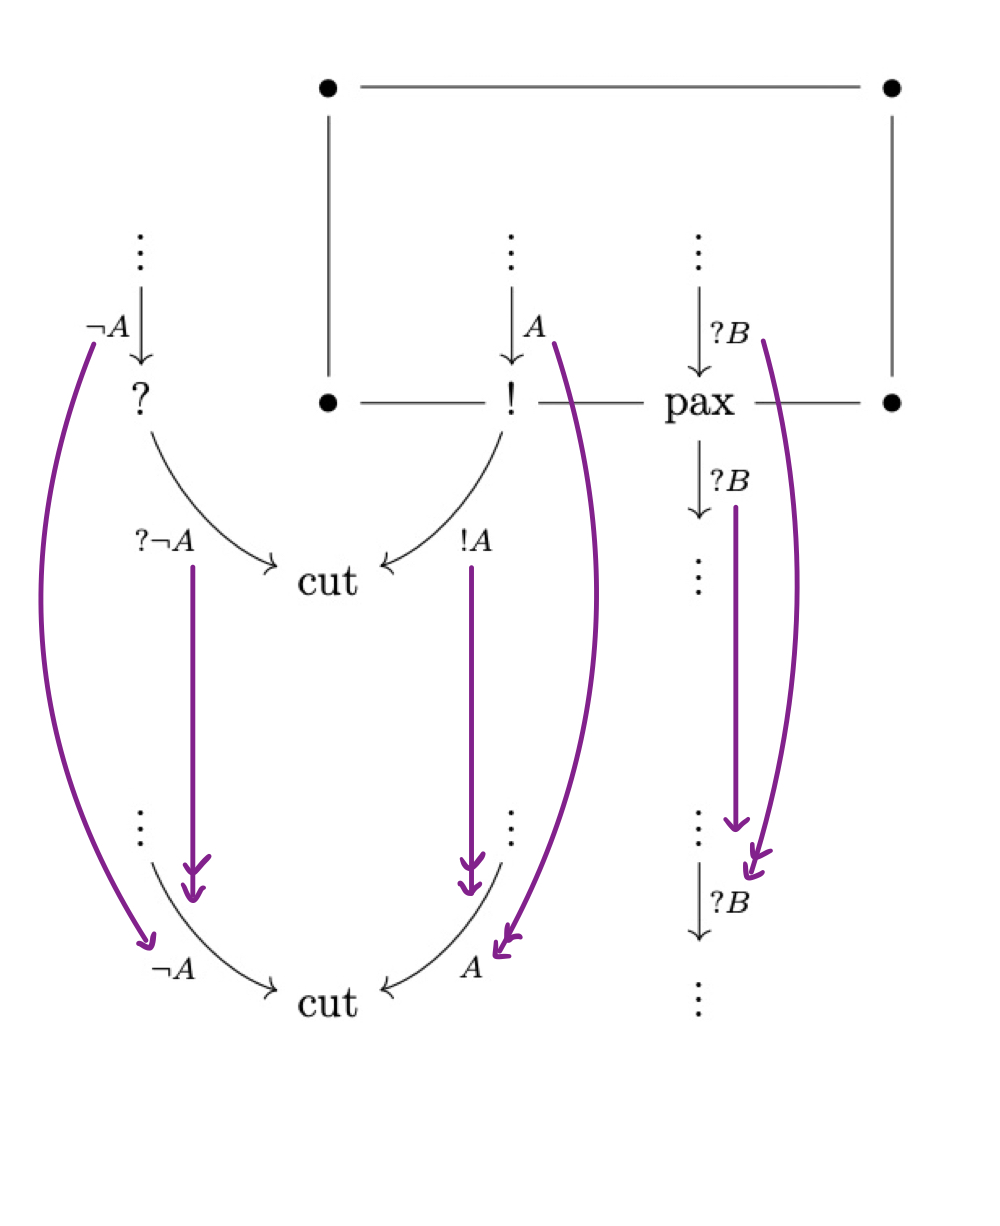
\includegraphics[width=0.5\textwidth]{DerS.jpeg}
\caption{$S_\gamma$ when $\gamma$ is a $!/?$-reduction}
\end{figure}
\item \textbf{$!/\pax$-reduction}:.
\begin{figure}[h]\label{fig:PaxS}
\centering
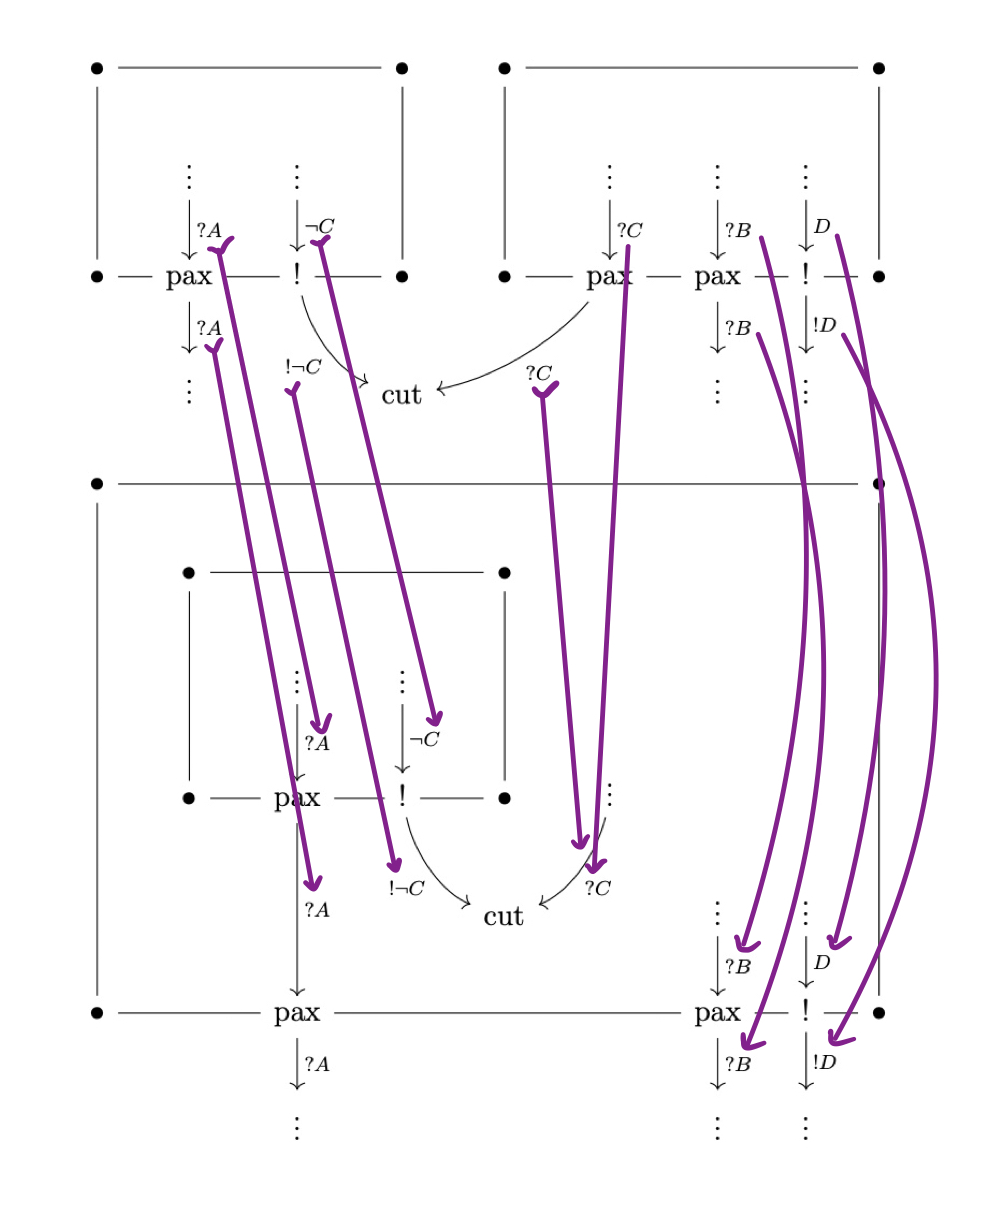
\includegraphics[width=0.5\textwidth]{PaxS.jpeg}
\caption{$S_\gamma$ when $\gamma$ is a $!/\pax$-reduction}
\end{figure}
The displayed maps are either the identity or involve mapping the unoriented atoms $\operatorname{Dep}U_E$ into $\bb{N} \times \operatorname{Dep}U_{E}$, for some formula $E$. These maps are given by inclusion; if $\textbf{X} \in \operatorname{Dep}U_{E}$ then the image under this map is $(0, \textbf{X})$. See Figure \ref{fig:PaxS}.

\item \textbf{$!/\weak$-reduction}. Consider \eqref{eq:pw_reduc_S}. The displayed occurrences of $?A, !\neg A$ have corresponding sets of unoriented atoms $\operatorname{Dep}U_{?A}, \operatorname{Dep}U_{!\neg A}$. There is a natural injection $P_{\pi'} \rightarrowtail P_\pi$, we let $S_\gamma$ be the retraction to this which maps the variables $\operatorname{Dep}U_{?A} \cup \operatorname{Dep}U_{!\neg A}$ in $P_{\pi}$ to $0 \in P_{\pi'}$.
% https://q.uiver.app/?q=WzAsMTEsWzIsMCwiXFx2ZG90cyJdLFsyLDEsIlxcYnVsbGV0Il0sWzEsMSwiXFxvcGVyYXRvcm5hbWV7d2t9Il0sWzAsMSwiXFxoZG90cyJdLFsxLDAsIlxccGkiXSxbMSwyLCI/QSJdLFsyLDMsIlxcb3BlcmF0b3JuYW1le2N1dH0iXSxbMywyLCIhIFxcbmVnIEEiXSxbMywxLCJcXHZkb3RzIl0sWzEsNCwiXFxwaSJdLFsyLDQsIjAiXSxbMiwzLCIiLDAseyJzdHlsZSI6eyJoZWFkIjp7Im5hbWUiOiJub25lIn19fV0sWzIsMSwiIiwyLHsic3R5bGUiOnsiaGVhZCI6eyJuYW1lIjoibm9uZSJ9fX1dLFswLDEsIiIsMCx7InN0eWxlIjp7ImhlYWQiOnsibmFtZSI6Im5vbmUifX19XSxbMiw1LCIiLDAseyJzdHlsZSI6eyJoZWFkIjp7Im5hbWUiOiJub25lIn19fV0sWzUsNiwiIiwwLHsiY3VydmUiOjJ9XSxbNyw2LCIiLDIseyJjdXJ2ZSI6LTJ9XSxbOCw3LCIiLDIseyJzdHlsZSI6eyJoZWFkIjp7Im5hbWUiOiJub25lIn19fV0sWzUsMTAsIiIsMCx7ImN1cnZlIjoyLCJjb2xvdXIiOlsyNzAsNjAsNjBdfV0sWzcsMTAsIiIsMCx7ImN1cnZlIjotMiwiY29sb3VyIjpbMjcwLDYwLDYwXX1dXQ==
\begin{equation}
\label{eq:pw_reduc_S}\begin{tikzcd}
	& & \vdots \\
	\hdots & {\operatorname{wk}} & \bullet & \vdots \\
	& {?A} && {! \neg A} \\
	&& {\operatorname{cut}} \\
	& & 0
	\arrow[line width=0.5mm, no head, from=2-2, to=2-1]
	\arrow[line width=0.5mm, no head, from=2-2, to=2-3]
	\arrow[line width=0.5mm, no head, from=1-3, to=2-3]
	\arrow[line width=0.5mm, no head, from=2-2, to=3-2]
	\arrow[curve={height=12pt}, from=3-2, to=4-3]
	\arrow[curve={height=-12pt}, from=3-4, to=4-3]
	\arrow[no head, from=2-4, to=3-4]
	\arrow[line width=0.5mm, color={rgb,255:red,153;green,92;blue,214}, curve={height=12pt}, from=3-2, to=5-3]
	\arrow[line width=0.5mm, color={rgb,255:red,153;green,92;blue,214}, curve={height=-12pt}, from=3-4, to=5-3]
\end{tikzcd}
\end{equation}
\item \textbf{$!/\ctr$-reduction}. Associated to the conclusion $?\neg A$ of the displayed contraction link in $\pi$ is a set of unoriented atoms $U_{?\neg A}$. Similarly for the two displayed occurrences of $? \neg A$ in $\pi'$.

There are two inclusion maps
\begin{equation}
\iota_1: P_{?\neg A} \lto P_{\pi'},\qquad \iota_2: P_{?\neg A} \lto P_{\pi'}
\end{equation}
We define a map $P_{?\neg A} \lto P_{\pi'}$ given by linearity along with the condition
\begin{equation}
(j, \mathbf{X}) \longmapsto
\begin{cases}
(j/2, \mathbf{X}),& j\text{ is even}\\
((j-1)/2, \mathbf{X}),& j\text{ is odd}
\end{cases}
\end{equation}
We do something similar for the displayed occurrences of $!A$ as well as all variables inside the box. This induces a morphism $S_\gamma: P_\pi \lto P_{\pi'}$. See Figure \ref{fig:CtrS}.
\begin{figure}[h]\label{fig:CtrS}
\centering
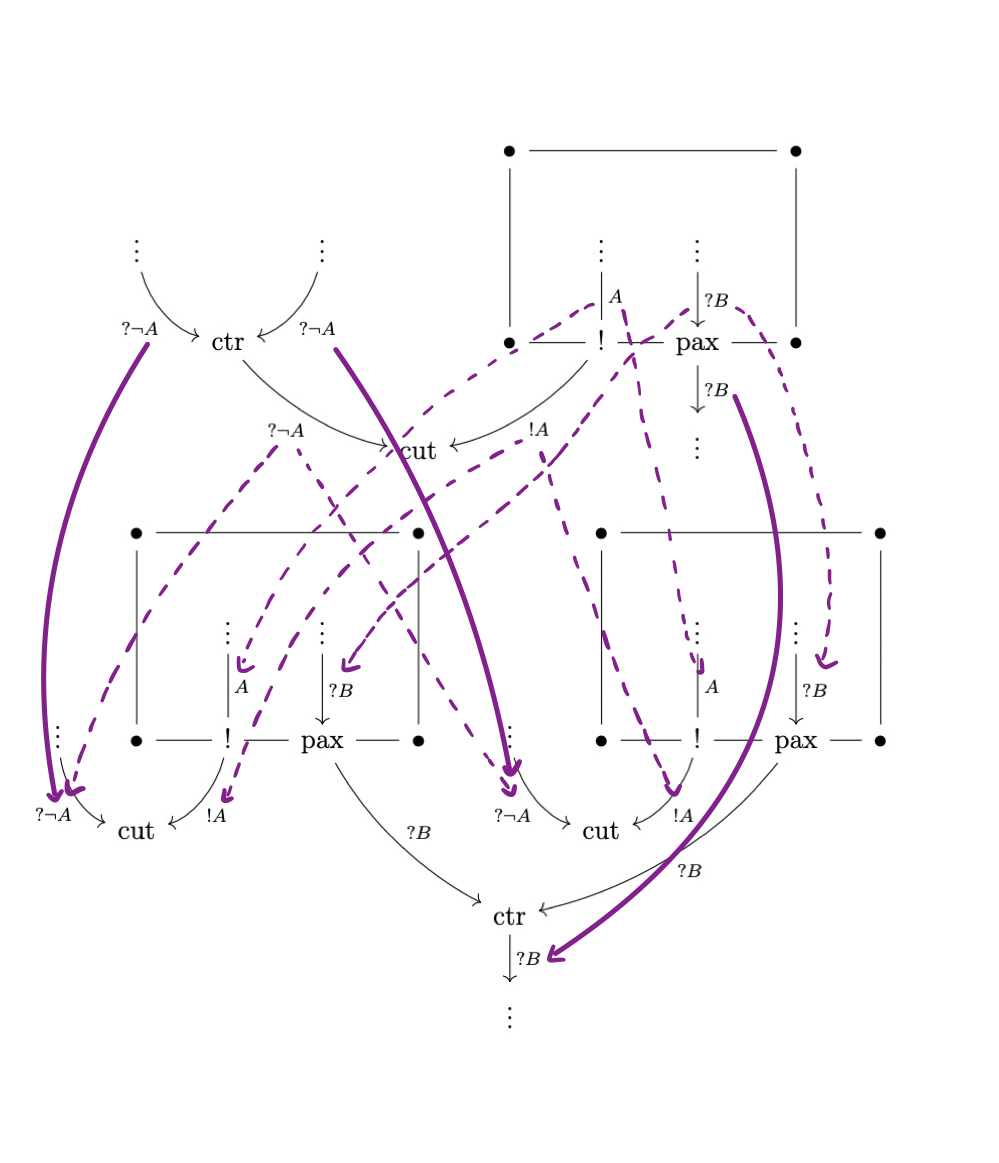
\includegraphics[width=0.5\textwidth]{CtrS.jpeg}
\caption{$S_\gamma$ when $\gamma$ is a $!/\ctr$-reduction.}
\end{figure}
\end{itemize}
\end{defn}
\begin{defn}
We extend the definition of $T_\gamma$ given in \cite[Definition 4.4]{AlgPnt}.
\begin{itemize}
\item \textbf{$!/?$-reduction $\gamma: \pi \lto \pi'$}. We notice that although these two occurrences have the same unoriented atoms $U_A$, they have different depth. Thus, we need to construct a function
\begin{equation}
\operatorname{Dep}U_A \lto \bb{N} \times \operatorname{Dep}U_A
\end{equation}
We take this to be
\begin{equation}
\mathbf{X} \longmapsto (0, \mathbf{X}).
\end{equation}
This induces a morphism $P_{\pi'}\lto P_\pi$, see Figure \ref{fig:DerT}.
\begin{figure}[h]\label{fig:DerT}
\centering
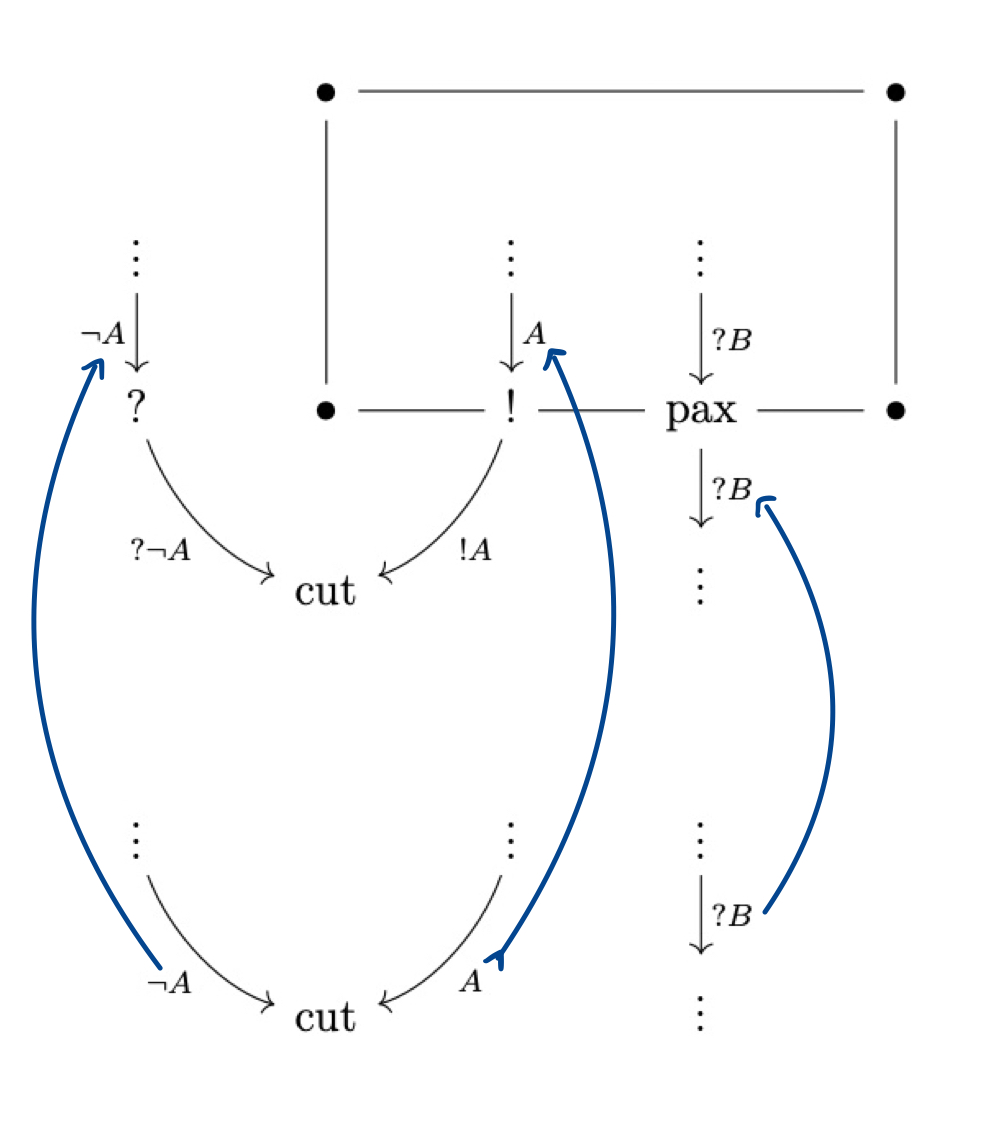
\includegraphics[width=0.5\textwidth]{DerT.jpeg}
\caption{$T_\gamma$ when $\gamma$ is a $!/?$-reduction.}
\end{figure}
\item \textbf{$!/\pax$-reduction}. The displayed maps in \ref{fig:PaxT} are either identities or inclusions $\textbf{X} \longmapsto (0, \textbf{X})$.
\begin{figure}[h]\label{fig:PaxT}
\centering
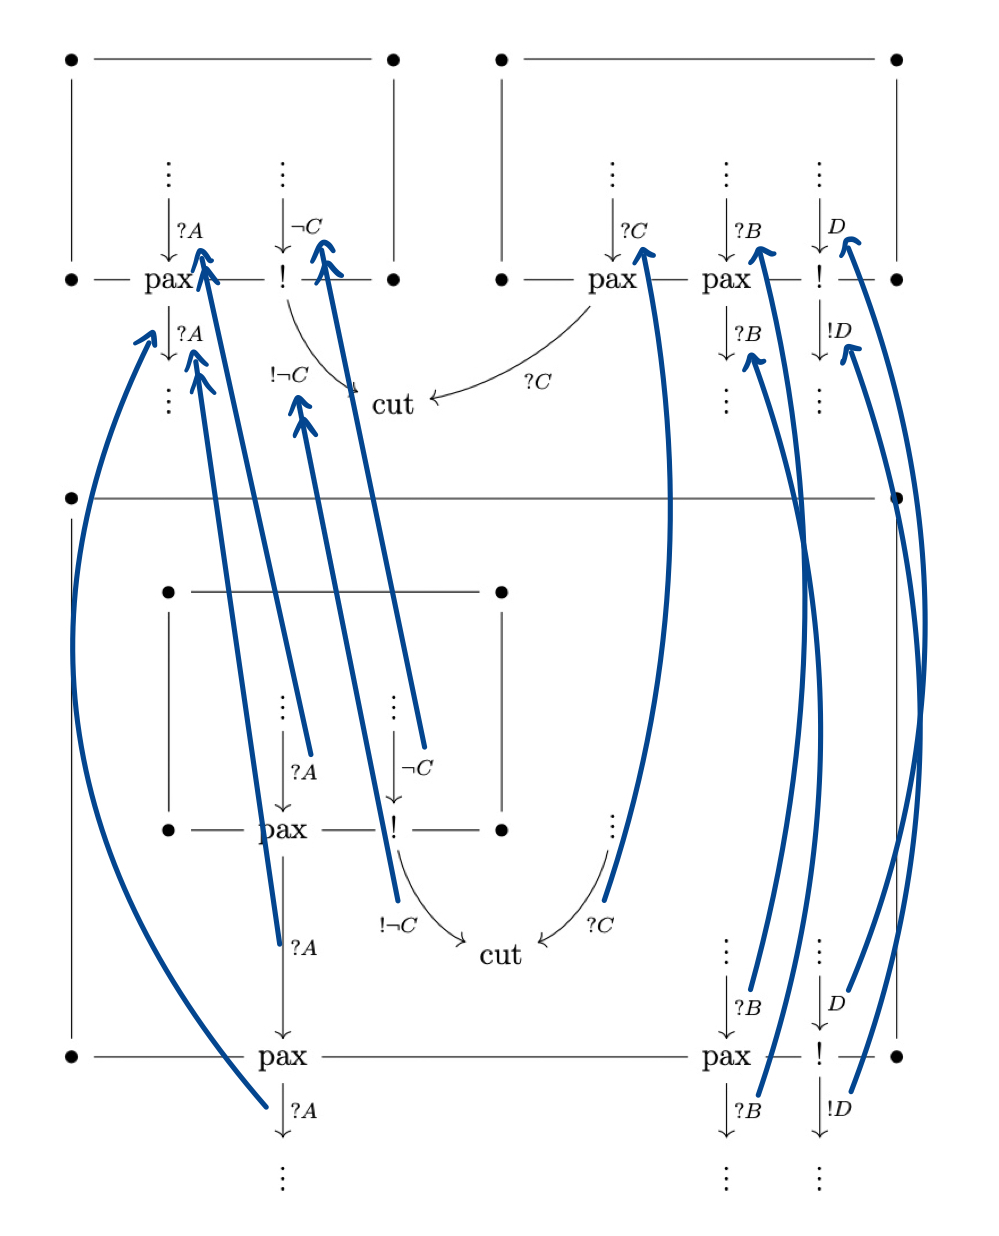
\includegraphics[width=0.5\textwidth]{PaxT.jpeg}
\caption{$T_\gamma$ when $\gamma$ is a $!/\pax$-reduction.}
\end{figure}
\item \textbf{$!/\weak$-reduction}.
% https://q.uiver.app/?q=WzAsMTIsWzIsMCwiXFx2ZG90cyJdLFsyLDEsIlxcYnVsbGV0Il0sWzEsMSwiXFxvcGVyYXRvcm5hbWV7d2t9Il0sWzAsMSwiXFxoZG90cyJdLFsxLDAsIlxccGkiXSxbMSwyLCI/QSJdLFsyLDMsIlxcb3BlcmF0b3JuYW1le2N1dH0iXSxbMywyLCIhIFxcbmVnIEEiXSxbMywxLCJcXHZkb3RzIl0sWzEsNCwiXFxwaSJdLFsyLDQsIjAiXSxbNCwyLCIwIl0sWzIsMywiIiwwLHsic3R5bGUiOnsiaGVhZCI6eyJuYW1lIjoibm9uZSJ9fX1dLFsyLDEsIiIsMix7InN0eWxlIjp7ImhlYWQiOnsibmFtZSI6Im5vbmUifX19XSxbMCwxLCIiLDAseyJzdHlsZSI6eyJoZWFkIjp7Im5hbWUiOiJub25lIn19fV0sWzIsNSwiIiwwLHsic3R5bGUiOnsiaGVhZCI6eyJuYW1lIjoibm9uZSJ9fX1dLFs1LDYsIiIsMCx7ImN1cnZlIjoyfV0sWzcsNiwiIiwyLHsiY3VydmUiOi0yfV0sWzgsNywiIiwyLHsic3R5bGUiOnsiaGVhZCI6eyJuYW1lIjoibm9uZSJ9fX1dLFsxMCwxMSwiIiwwLHsiY3VydmUiOjIsImNvbG91ciI6WzI0MCw2MCw2MF19XV0=
\begin{equation}
\label{eq:d_redex_T}
\begin{tikzcd}
	& \zeta & \vdots \\
	\hdots & {\operatorname{wk}} & \bullet & \vdots \\
	& {?A} && {! \neg A} & 0 \\
	&& {\operatorname{cut}} \\
	& \zeta & 0
	\arrow[line width=0.5mm,no head, from=2-2, to=2-1]
	\arrow[line width=0.5mm,no head, from=2-2, to=2-3]
	\arrow[line width=0.5mm,no head, from=1-3, to=2-3]
	\arrow[no head, from=2-2, to=3-2]
	\arrow[curve={height=12pt}, from=3-2, to=4-3]
	\arrow[curve={height=-12pt}, from=3-4, to=4-3]
	\arrow[no head, from=2-4, to=3-4]
	\arrow[line width=0.55mm,color={rgb,255:red,92;green,92;blue,214}, curve={height=12pt}, from=5-3, to=3-5]
\end{tikzcd}
\end{equation}
This map is the obvious inclusion $P_{\pi'} \rightarrowtail P_{\pi}$.
\item \textbf{$!/\ctr$-reduction}. Recall that $U_{!A} = \bb{N} \times U_A$. We consider the two maps
\begin{align*}
U_{!A} &\lto U_{!A}\\
(j, \mathbf{X}) &\longmapsto (2j, \mathbf{X})\\
U_{!A} &\lto U_{!A}\\
(j, \mathbf{X}) &\longmapsto (2j + 1, \mathbf{X})
\end{align*}
\end{itemize}
\begin{figure}[h]\label{fig:CtrT}
\centering
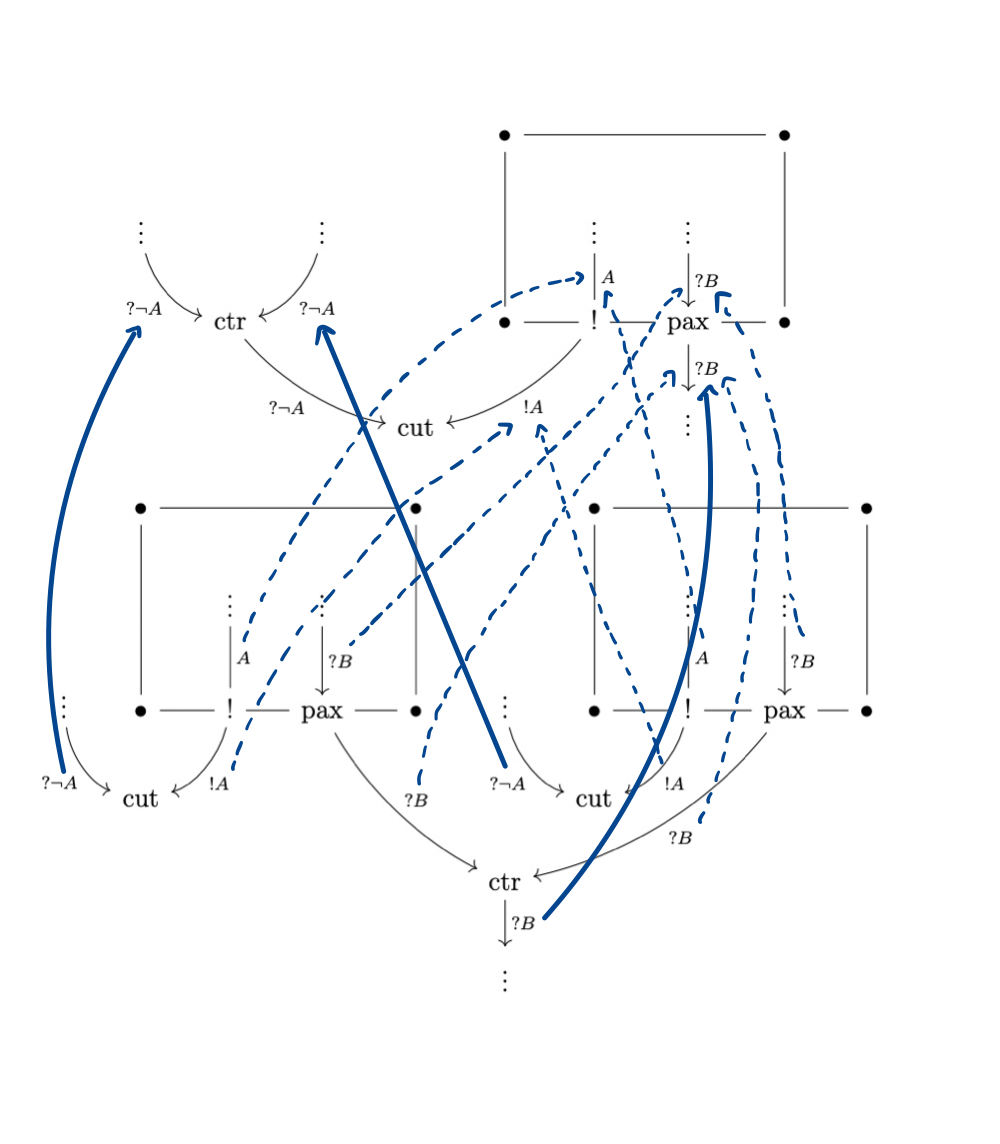
\includegraphics[width=0.5\textwidth]{CtrT.jpeg}
\caption{$S_\gamma$ when $\gamma$ is a $!/\ctr$-reduction.}
\end{figure}
We use this to include two boxes into one. See Figure \ref{fig:CtrT}.
\end{defn}

\section{Geometry of Interaction Zero, Exponentials}

Now we prove the extension of \cite[Proposition 4.6]{MT}. Recall from the statement of that proposition what it means to have a morphism of pairs consisting of a polynomial ring and an ideal.

\begin{lemma}\label{lem:global_equivalence}
Consider a $p$-redex inside a proof net $\pi$.
% https://q.uiver.app/?q=WzAsMjIsWzEsMSwiXFx2ZG90cyJdLFsxLDIsIlxcb3BlcmF0b3JuYW1le3BheH0iXSxbMiwyLCIhIl0sWzMsMiwiXFxidWxsZXQiXSxbMCwyLCJcXGJ1bGxldCJdLFs0LDIsIlxcYnVsbGV0Il0sWzUsMiwiXFxvcGVyYXRvcm5hbWV7cGF4fSJdLFs2LDIsIlxcb3BlcmF0b3JuYW1le3BheH0iXSxbNywyLCIhIl0sWzgsMiwiXFxidWxsZXQiXSxbNywxLCJcXHZkb3RzIl0sWzYsMSwiXFx2ZG90cyJdLFs1LDEsIlxcdmRvdHMiXSxbMiwxLCJcXHZkb3RzIl0sWzAsMCwiXFxidWxsZXQiXSxbMywwLCJcXGJ1bGxldCJdLFsxLDMsIlxcdmRvdHMiXSxbNiwzLCJcXHZkb3RzIl0sWzcsMywiXFx2ZG90cyJdLFs0LDAsIlxcYnVsbGV0Il0sWzgsMCwiXFxidWxsZXQiXSxbMywzLCJcXG9wZXJhdG9ybmFtZXtjdXR9Il0sWzE0LDQsIiIsMCx7InN0eWxlIjp7ImhlYWQiOnsibmFtZSI6Im5vbmUifX19XSxbMTQsMTUsIiIsMix7InN0eWxlIjp7ImhlYWQiOnsibmFtZSI6Im5vbmUifX19XSxbMTUsMywiIiwyLHsic3R5bGUiOnsiaGVhZCI6eyJuYW1lIjoibm9uZSJ9fX1dLFszLDIsIiIsMix7InN0eWxlIjp7ImhlYWQiOnsibmFtZSI6Im5vbmUifX19XSxbMSw0LCIiLDIseyJzdHlsZSI6eyJoZWFkIjp7Im5hbWUiOiJub25lIn19fV0sWzE5LDUsIiIsMix7InN0eWxlIjp7ImhlYWQiOnsibmFtZSI6Im5vbmUifX19XSxbNSw2LCIiLDIseyJzdHlsZSI6eyJoZWFkIjp7Im5hbWUiOiJub25lIn19fV0sWzcsOCwiIiwyLHsic3R5bGUiOnsiaGVhZCI6eyJuYW1lIjoibm9uZSJ9fX1dLFs4LDksIiIsMix7InN0eWxlIjp7ImhlYWQiOnsibmFtZSI6Im5vbmUifX19XSxbOSwyMCwiIiwyLHsic3R5bGUiOnsiaGVhZCI6eyJuYW1lIjoibm9uZSJ9fX1dLFsxOSwyMCwiIiwwLHsic3R5bGUiOnsiaGVhZCI6eyJuYW1lIjoibm9uZSJ9fX1dLFswLDEsIj9BIl0sWzEsMTYsIj9BIl0sWzEzLDIsIlxcbmVnIEMiXSxbNiwyMSwiPyBDIiwwLHsiY3VydmUiOi0yfV0sWzIsMjEsIiFcXG5lZyBDIiwyLHsiY3VydmUiOjJ9XSxbMTIsNiwiP0MiXSxbMTEsNywiP0IiXSxbNywxNywiP0IiXSxbMTAsOCwiRCJdLFs4LDE4LCIhRCJdLFsxLDIsIiIsMSx7InN0eWxlIjp7ImhlYWQiOnsibmFtZSI6Im5vbmUifX19XSxbNiw3LCIiLDAseyJzdHlsZSI6eyJoZWFkIjp7Im5hbWUiOiJub25lIn19fV1d
\begin{equation}\label{eq:p_redex_lemma}
\begin{tikzcd}[column sep = small]
	\bullet &&& \bullet & \bullet &&&& \bullet \\
	& \vdots & \vdots &&& \vdots & \vdots & \vdots \\
	\bullet & {\operatorname{pax}} & {!} & \bullet & \bullet & {\operatorname{pax}} & {\operatorname{pax}} & {!} & \bullet \\
	& \vdots && {\operatorname{cut}} &&& \vdots & \vdots
	\arrow[no head, from=1-1, to=3-1]
	\arrow[no head, from=1-1, to=1-4]
	\arrow[no head, from=1-4, to=3-4]
	\arrow[no head, from=3-4, to=3-3]
	\arrow[no head, from=3-2, to=3-1]
	\arrow[no head, from=1-5, to=3-5]
	\arrow[no head, from=3-5, to=3-6]
	\arrow[no head, from=3-7, to=3-8]
	\arrow[no head, from=3-8, to=3-9]
	\arrow[no head, from=3-9, to=1-9]
	\arrow[no head, from=1-5, to=1-9]
	\arrow["{?A}", from=2-2, to=3-2]
	\arrow["{?A}", from=3-2, to=4-2]
	\arrow["{\neg C}", from=2-3, to=3-3]
	\arrow["{? C}", curve={height=-12pt}, from=3-6, to=4-4]
	\arrow["{!\neg C}"', curve={height=12pt}, from=3-3, to=4-4]
	\arrow["{?C}", from=2-6, to=3-6]
	\arrow["{?B}", from=2-7, to=3-7]
	\arrow["{?B}", from=3-7, to=4-7]
	\arrow["D", from=2-8, to=3-8]
	\arrow["{!D}", from=3-8, to=4-8]
	\arrow[no head, from=3-2, to=3-3]
	\arrow[no head, from=3-6, to=3-7]
\end{tikzcd}
\end{equation}
If the $\cut$-link of connecting the two boxes in the $p$-redex has presmises $! \neg C, ?C$ then let $?A_1, \ldots, ?A_n$ denote the conclusions to the $\pax$-links of the box which promotes $\neg C$, and let $?B_1, \ldots, ?B_m$ denote the conclusions to the $\pax$-links of the other box. (In \eqref{eq:p_redex_lemma} the case $n = m = 1$ is shown).

Assume that all conclusions to all axiom links of $\pi$ are atomic. Let $\mathbf{X}$ be an arbitrary element of $\operatorname{Dep}U_{\neg C}$. Then one of the following hold.
\begin{itemize}
	\item $\mathbf{X} \sim 0$.
	\item There exists $1 \leq k \leq m$ and $\mathbf{X}' \in \operatorname{Dep}U_{?B_k}$ such that $\mathbf{X} \sim \mathbf{X}'$.
	\item There exists $1 \leq k \leq n$ and $\mathbf{X}' \in \operatorname{Dep}U_{?A_k}$ such that $\mathbf{X} \sim \mathbf{X}'$.
	\item There exists $\mathbf{X'} \in \operatorname{Dep}U_{D}$ such that $\mathbf{X} \sim \mathbf{X}'$.
\end{itemize}
\end{lemma}
\begin{proof}
First we perform a $!/\pax$-reduction.
% https://q.uiver.app/?q=WzAsMjIsWzEsMSwiXFxidWxsZXQiXSxbMSwzLCJcXGJ1bGxldCJdLFs0LDMsIlxcYnVsbGV0Il0sWzQsMSwiXFxidWxsZXQiXSxbMiwyLCJcXHZkb3RzIl0sWzMsMiwiXFx2ZG90cyJdLFszLDMsIiEiXSxbMiwzLCJcXG9wZXJhdG9ybmFtZXtwYXh9Il0sWzQsNCwiXFxvcGVyYXRvcm5hbWV7Y3V0fSJdLFs1LDMsIlxcdmRvdHMiXSxbNiw0LCJcXHZkb3RzIl0sWzcsNCwiXFx2ZG90cyJdLFs2LDUsIlxcb3BlcmF0b3JuYW1le3BheH0iXSxbNyw1LCIhIl0sWzIsNSwiXFxvcGVyYXRvcm5hbWV7cGF4fSJdLFswLDUsIlxcYnVsbGV0Il0sWzAsMCwiXFxidWxsZXQiXSxbOCwwLCJcXGJ1bGxldCJdLFs4LDUsIlxcYnVsbGV0Il0sWzcsNiwiXFx2ZG90cyJdLFs2LDYsIlxcdmRvdHMiXSxbMiw2LCJcXHZkb3RzIl0sWzAsMSwiIiwwLHsic3R5bGUiOnsiaGVhZCI6eyJuYW1lIjoibm9uZSJ9fX1dLFswLDMsIiIsMix7InN0eWxlIjp7ImhlYWQiOnsibmFtZSI6Im5vbmUifX19XSxbMywyLCIiLDIseyJzdHlsZSI6eyJoZWFkIjp7Im5hbWUiOiJub25lIn19fV0sWzEsNywiIiwwLHsic3R5bGUiOnsiaGVhZCI6eyJuYW1lIjoibm9uZSJ9fX1dLFs2LDIsIiIsMCx7InN0eWxlIjp7ImhlYWQiOnsibmFtZSI6Im5vbmUifX19XSxbNSw2LCJcXG5lZyBDIl0sWzQsNywiP0EiXSxbOSw4LCI/QyIsMCx7ImN1cnZlIjotMn1dLFs2LDgsIiFcXG5lZyBDIiwyLHsiY3VydmUiOjJ9XSxbNywxNCwiP0EiXSxbMTAsMTIsIj9CIl0sWzExLDEzLCJEIl0sWzE4LDEzLCIiLDIseyJzdHlsZSI6eyJoZWFkIjp7Im5hbWUiOiJub25lIn19fV0sWzEzLDEyLCIiLDIseyJzdHlsZSI6eyJoZWFkIjp7Im5hbWUiOiJub25lIn19fV0sWzE4LDE3LCIiLDAseyJzdHlsZSI6eyJoZWFkIjp7Im5hbWUiOiJub25lIn19fV0sWzE3LDE2LCIiLDAseyJzdHlsZSI6eyJoZWFkIjp7Im5hbWUiOiJub25lIn19fV0sWzE2LDE1LCIiLDAseyJzdHlsZSI6eyJoZWFkIjp7Im5hbWUiOiJub25lIn19fV0sWzE1LDE0LCIiLDEseyJzdHlsZSI6eyJoZWFkIjp7Im5hbWUiOiJub25lIn19fV0sWzEyLDIwLCI/QiJdLFsxMywxOSwiIUQiXSxbMTQsMjEsIj9BIl0sWzE0LDEyLCIiLDAseyJzdHlsZSI6eyJoZWFkIjp7Im5hbWUiOiJub25lIn19fV0sWzcsNiwiIiwxLHsic3R5bGUiOnsiaGVhZCI6eyJuYW1lIjoibm9uZSJ9fX1dXQ==
\[\begin{tikzcd}[column sep = small]
	\bullet &&&&&&&& \bullet \\
	& \bullet &&& \bullet \\
	&& \vdots & \vdots \\
	& \bullet & {\operatorname{pax}} & {!} & \bullet & \vdots \\
	&&&& {\operatorname{cut}} && \vdots & \vdots \\
	\bullet && {\operatorname{pax}} &&&& {\operatorname{pax}} & {!} & \bullet \\
	&& \vdots &&&& \vdots & \vdots
	\arrow[no head, from=2-2, to=4-2]
	\arrow[no head, from=2-2, to=2-5]
	\arrow[no head, from=2-5, to=4-5]
	\arrow[no head, from=4-2, to=4-3]
	\arrow[no head, from=4-4, to=4-5]
	\arrow["{\neg C}", from=3-4, to=4-4]
	\arrow["{?A}", from=3-3, to=4-3]
	\arrow["{?C}", curve={height=-12pt}, from=4-6, to=5-5]
	\arrow["{!\neg C}"', curve={height=12pt}, from=4-4, to=5-5]
	\arrow["{?A}", from=4-3, to=6-3]
	\arrow["{?B}", from=5-7, to=6-7]
	\arrow["D", from=5-8, to=6-8]
	\arrow[no head, from=6-9, to=6-8]
	\arrow[no head, from=6-8, to=6-7]
	\arrow[no head, from=6-9, to=1-9]
	\arrow[no head, from=1-9, to=1-1]
	\arrow[no head, from=1-1, to=6-1]
	\arrow[no head, from=6-1, to=6-3]
	\arrow["{?B}", from=6-7, to=7-7]
	\arrow["{!D}", from=6-8, to=7-8]
	\arrow["{?A}", from=6-3, to=7-3]
	\arrow[no head, from=6-3, to=6-7]
	\arrow[no head, from=4-3, to=4-4]
\end{tikzcd}\]
Let $\pi'$ denote the result. By observation of this reduction rule, we see that this Lemma holds true if and only if one of the following statements holds:
\begin{itemize}
	\item $T(\textbf{X}) \sim 0$.
	\item There exists $1 \leq k \leq m$ and $X' \in \operatorname{Dep}U_{?B_k}$, where $?B_k$ is the premise to a $\pax$ door of the displayed outer box, such that $T(\textbf{X}) \sim \textbf{X}'$.
	\item There exists $1 \leq k \leq n$ and $X' \in \operatorname{Dep}U_{?A_k}$, where $?A_k$ is the premise to a $\pax$ door of the displayed inner box, such that $T(\mathbf{X}) \sim \mathbf{X}'$.
	\item There exists $\textbf{X}' \in \operatorname{Dep}U_{D}$ such that $T(\textbf{X}) \sim \textbf{X}'$.
\end{itemize}
Thus we only need to consider the following subproof.
% https://q.uiver.app/?q=WzAsMTUsWzAsMCwiXFxidWxsZXQiXSxbMCwyLCJcXGJ1bGxldCJdLFszLDIsIlxcYnVsbGV0Il0sWzMsMCwiXFxidWxsZXQiXSxbMSwxLCJcXHZkb3RzIl0sWzIsMSwiXFx2ZG90cyJdLFsyLDIsIiEiXSxbMSwyLCJcXG9wZXJhdG9ybmFtZXtwYXh9Il0sWzMsMywiXFxvcGVyYXRvcm5hbWV7Y3V0fSJdLFs0LDIsIlxcdmRvdHMiXSxbNSwyLCJcXHZkb3RzIl0sWzYsMiwiXFx2ZG90cyJdLFs1LDMsIlxcdmRvdHMiXSxbNiwzLCJcXHZkb3RzIl0sWzEsMywiXFx2ZG90cyJdLFswLDEsIiIsMCx7InN0eWxlIjp7ImhlYWQiOnsibmFtZSI6Im5vbmUifX19XSxbMCwzLCIiLDIseyJzdHlsZSI6eyJoZWFkIjp7Im5hbWUiOiJub25lIn19fV0sWzMsMiwiIiwyLHsic3R5bGUiOnsiaGVhZCI6eyJuYW1lIjoibm9uZSJ9fX1dLFsxLDcsIiIsMCx7InN0eWxlIjp7ImhlYWQiOnsibmFtZSI6Im5vbmUifX19XSxbNiwyLCIiLDAseyJzdHlsZSI6eyJoZWFkIjp7Im5hbWUiOiJub25lIn19fV0sWzUsNiwiXFxuZWcgQyJdLFs0LDcsIj9BIl0sWzksOCwiP0MiLDAseyJjdXJ2ZSI6LTJ9XSxbNiw4LCIhXFxuZWcgQyIsMix7ImN1cnZlIjoyfV0sWzEwLDEyLCI/QiJdLFsxMSwxMywiRCJdLFs3LDE0LCI/QSJdLFs3LDYsIiIsMSx7InN0eWxlIjp7ImhlYWQiOnsibmFtZSI6Im5vbmUifX19XV0=
\[\begin{tikzcd}
	\bullet &&& \bullet \\
	& \vdots & \vdots \\
	\bullet & {\operatorname{pax}} & {!} & \bullet & \vdots & \vdots & \vdots \\
	& \vdots && {\operatorname{cut}} && \vdots & \vdots
	\arrow[no head, from=1-1, to=3-1]
	\arrow[no head, from=1-1, to=1-4]
	\arrow[no head, from=1-4, to=3-4]
	\arrow[no head, from=3-1, to=3-2]
	\arrow[no head, from=3-3, to=3-4]
	\arrow["{\neg C}", from=2-3, to=3-3]
	\arrow["{?A}", from=2-2, to=3-2]
	\arrow["{?C}", curve={height=-12pt}, from=3-5, to=4-4]
	\arrow["{!\neg C}"', curve={height=12pt}, from=3-3, to=4-4]
	\arrow["{?B}", from=3-6, to=4-6]
	\arrow["D", from=3-7, to=4-7]
	\arrow["{?A}", from=3-2, to=4-2]
	\arrow[no head, from=3-2, to=3-3]
\end{tikzcd}\]
Let $l$ denote the link to which the displayed $?C$ edge is conclusion inside $\pi'$. By the structure of $?C$ we have that $l$ is one of $\ctr, \pax, \weak, ?$ (note that $l$ cannot be $\ax$ because we have assumed that the conclusions to all $\ax$-links in $\pi$ are atomic).

If $l$ is $\weak$ then $\mathbf{X} \sim 0$ and we are done.

If $l$ is $\pax$ then perform another $!/\pax$-reduction. The statement of this Lemma then reduces similarly to already shown.

If $l = \ctr$, we perform a $!/\ctr$-reduction and observe that this duplicates the box which promotes the displayed $\neg C$ formula. This results in the following, where we have only drawn the $n = m = 1$ case.
% https://q.uiver.app/?q=WzAsMjYsWzUsMCwiXFxidWxsZXQiXSxbNSwyLCJcXGJ1bGxldCJdLFs4LDIsIlxcYnVsbGV0Il0sWzgsMCwiXFxidWxsZXQiXSxbNiwxLCJcXHZkb3RzIl0sWzcsMSwiXFx2ZG90cyJdLFs3LDIsIiEiXSxbNiwyLCJcXG9wZXJhdG9ybmFtZXtwYXh9Il0sWzgsMywiXFxvcGVyYXRvcm5hbWV7Y3V0fSJdLFs5LDIsIlxcdmRvdHMiXSxbMTAsMiwiXFx2ZG90cyJdLFsxMSwyLCJcXHZkb3RzIl0sWzEwLDMsIlxcdmRvdHMiXSxbMTEsMywiXFx2ZG90cyJdLFszLDIsIlxcYnVsbGV0Il0sWzMsMCwiXFxidWxsZXQiXSxbMCwwLCJcXGJ1bGxldCJdLFswLDIsIlxcYnVsbGV0Il0sWzEsMiwiXFxvcGVyYXRvcm5hbWV7cGF4fSJdLFsyLDIsIiEiXSxbNCwyLCJcXHZkb3RzIl0sWzMsMywiXFxvcGVyYXRvcm5hbWV7Y3V0fSJdLFs0LDQsIlxcb3BlcmF0b3JuYW1le2N0cn0iXSxbNCw1LCJcXHZkb3RzIl0sWzEsMSwiXFx2ZG90cyJdLFsyLDEsIlxcdmRvdHMiXSxbMCwxLCIiLDAseyJzdHlsZSI6eyJoZWFkIjp7Im5hbWUiOiJub25lIn19fV0sWzAsMywiIiwyLHsic3R5bGUiOnsiaGVhZCI6eyJuYW1lIjoibm9uZSJ9fX1dLFszLDIsIiIsMix7InN0eWxlIjp7ImhlYWQiOnsibmFtZSI6Im5vbmUifX19XSxbNyw2LCIiLDAseyJzdHlsZSI6eyJoZWFkIjp7Im5hbWUiOiJub25lIn19fV0sWzYsMiwiIiwwLHsic3R5bGUiOnsiaGVhZCI6eyJuYW1lIjoibm9uZSJ9fX1dLFs1LDYsIlxcbmVnIEMiXSxbNCw3LCI/QSJdLFs5LDgsIj9DIiwwLHsiY3VydmUiOi0yfV0sWzYsOCwiIVxcbmVnIEMiLDIseyJjdXJ2ZSI6Mn1dLFsxMCwxMiwiP0IiXSxbMTEsMTMsIkQiXSxbMSw3LCIiLDAseyJzdHlsZSI6eyJoZWFkIjp7Im5hbWUiOiJub25lIn19fV0sWzE2LDE1LCIiLDAseyJzdHlsZSI6eyJoZWFkIjp7Im5hbWUiOiJub25lIn19fV0sWzE1LDE0LCIiLDAseyJzdHlsZSI6eyJoZWFkIjp7Im5hbWUiOiJub25lIn19fV0sWzE5LDIxLCIhXFxuZWcgQyIsMix7ImN1cnZlIjoyfV0sWzIwLDIxLCI/QyIsMCx7ImN1cnZlIjotMn1dLFs3LDIyLCI/QSIsMCx7ImN1cnZlIjotMn1dLFsxOCwyMiwiP0EiLDIseyJjdXJ2ZSI6NH1dLFsyMiwyMywiP0EiXSxbMTcsMTgsIiIsMix7InN0eWxlIjp7ImhlYWQiOnsibmFtZSI6Im5vbmUifX19XSxbMTgsMTksIiIsMix7InN0eWxlIjp7ImhlYWQiOnsibmFtZSI6Im5vbmUifX19XSxbMTksMTQsIiIsMix7InN0eWxlIjp7ImhlYWQiOnsibmFtZSI6Im5vbmUifX19XSxbMTYsMTcsIiIsMix7InN0eWxlIjp7ImhlYWQiOnsibmFtZSI6Im5vbmUifX19XSxbMjUsMTksIlxcbmVnIEMiXSxbMjQsMTgsIj9BIl1d
\[\begin{tikzcd}[column sep = small]
	\bullet &&& \bullet && \bullet &&& \bullet \\
	& \vdots & \vdots &&&& \vdots & \vdots \\
	\bullet & {\operatorname{pax}} & {!} & \bullet & \vdots & \bullet & {\operatorname{pax}} & {!} & \bullet & \vdots & \vdots & \vdots \\
	&&& {\operatorname{cut}} &&&&& {\operatorname{cut}} && \vdots & \vdots \\
	&&&& {\operatorname{ctr}} \\
	&&&& \vdots
	\arrow[no head, from=1-6, to=3-6]
	\arrow[no head, from=1-6, to=1-9]
	\arrow[no head, from=1-9, to=3-9]
	\arrow[no head, from=3-7, to=3-8]
	\arrow[no head, from=3-8, to=3-9]
	\arrow["{\neg C}", from=2-8, to=3-8]
	\arrow["{?A}", from=2-7, to=3-7]
	\arrow["{?C}", curve={height=-12pt}, from=3-10, to=4-9]
	\arrow["{!\neg C}"', curve={height=12pt}, from=3-8, to=4-9]
	\arrow["{?B}", from=3-11, to=4-11]
	\arrow["D", from=3-12, to=4-12]
	\arrow[no head, from=3-6, to=3-7]
	\arrow[no head, from=1-1, to=1-4]
	\arrow[no head, from=1-4, to=3-4]
	\arrow["{!\neg C}"', curve={height=12pt}, from=3-3, to=4-4]
	\arrow["{?C}", curve={height=-12pt}, from=3-5, to=4-4]
	\arrow["{?A}", curve={height=-12pt}, from=3-7, to=5-5]
	\arrow["{?A}"', curve={height=24pt}, from=3-2, to=5-5]
	\arrow["{?A}", from=5-5, to=6-5]
	\arrow[no head, from=3-1, to=3-2]
	\arrow[no head, from=3-2, to=3-3]
	\arrow[no head, from=3-3, to=3-4]
	\arrow[no head, from=1-1, to=3-1]
	\arrow["{\neg C}", from=2-3, to=3-3]
	\arrow["{?A}", from=2-2, to=3-2]
\end{tikzcd}\]
The formula $\mathbf{X}$ is of the form $(n, \mathbf{X}')$ form some $n \in \bb{N}$ and some $\mathbf{X} \in \operatorname{Dep}U_{C}$. Whether $n$ is even or odd, the statement of the Lemma again reduces as already seen. Visually, the problem reduces to considering the left displayed box if $n$ is even, and to the right displayed box if $n$ is odd.

Thus it remains to consider the case where $l = ?$. We perform a $!/?$-reduction and obtain the following proof.
% https://q.uiver.app/?q=WzAsOSxbMiwxLCJcXG9wZXJhdG9ybmFtZXtjdXR9Il0sWzEsMCwiXFx2ZG90cyJdLFszLDAsIlxcdmRvdHMiXSxbMCwxLCJcXHZkb3RzIl0sWzQsMSwiXFx2ZG90cyJdLFs1LDEsIlxcdmRvdHMiXSxbMCwyLCJcXHZkb3RzIl0sWzQsMiwiXFx2ZG90cyJdLFs1LDIsIlxcdmRvdHMiXSxbMSwwLCJcXG5lZyBDIiwyLHsiY3VydmUiOjJ9XSxbMiwwLCJDIiwwLHsiY3VydmUiOi0yfV0sWzMsNiwiP0EiXSxbNCw3LCI/QiJdLFs1LDgsIkQiXV0=
\[\begin{tikzcd}
	& \vdots && \vdots \\
	\vdots && {\operatorname{cut}} && \vdots & \vdots \\
	\vdots &&&& \vdots & \vdots
	\arrow["{\neg C}"', curve={height=12pt}, from=1-2, to=2-3]
	\arrow["C", curve={height=-12pt}, from=1-4, to=2-3]
	\arrow["{?A}", from=2-1, to=3-1]
	\arrow["{?B}", from=2-5, to=3-5]
	\arrow["D", from=2-6, to=3-6]
\end{tikzcd}\]
Let $\zeta$ denote this proof. We prove the result in the case where $C$ is atomic, the general case reduces to this. Let $l_1, l_2$ denote respectively the link with conclusion the displayed $\neg C, C$ formulas. Since $C$ is atmoic, both $l_1, l_2$ are axiom links. Thus we have the following proof.
% https://q.uiver.app/?q=WzAsMTEsWzMsMSwiXFxvcGVyYXRvcm5hbWV7Y3V0fSJdLFsyLDAsIlxcb3BlcmF0b3JuYW1le2F4fSJdLFs0LDAsIlxcb3BlcmF0b3JuYW1le2F4fSJdLFswLDEsIlxcdmRvdHMiXSxbNiwxLCJcXHZkb3RzIl0sWzcsMSwiXFx2ZG90cyJdLFswLDIsIlxcdmRvdHMiXSxbNiwyLCJcXHZkb3RzIl0sWzcsMiwiXFx2ZG90cyJdLFs1LDEsIlxcdmRvdHMiXSxbMSwxLCJcXHZkb3RzIl0sWzMsNiwiP0EiXSxbNCw3LCI/QiJdLFs1LDgsIkQiXSxbMiw5LCJcXG5lZyBDIiwwLHsiY3VydmUiOi0yfV0sWzIsMCwiQyIsMl0sWzEsMCwiXFxuZWcgQyJdLFsxLDEwLCJDIiwyLHsiY3VydmUiOjJ9XV0=
\[\begin{tikzcd}
	&& {\operatorname{ax}} && {\operatorname{ax}} \\
	\vdots & \vdots && {\operatorname{cut}} && \vdots & \vdots & \vdots \\
	\vdots &&&&&& \vdots & \vdots
	\arrow["{?A}", from=2-1, to=3-1]
	\arrow["{?B}", from=2-7, to=3-7]
	\arrow["D", from=2-8, to=3-8]
	\arrow["{\neg C}", curve={height=-12pt}, from=1-5, to=2-6]
	\arrow["C"', from=1-5, to=2-4]
	\arrow["{\neg C}", from=1-3, to=2-4]
	\arrow["C"', curve={height=12pt}, from=1-3, to=2-2]
\end{tikzcd}\]
Follow the path starting at the $\neg C$ conclusion of the rightmost displayed $\ax$-link until we either reach a conclusion or a cut link. If we reach a conclusion, then we are done. If we reach a cut link, then reduce this cut link as far as possible without reducing any $\ax/\cut$ links. Do the same for the $C$ conclusion of the leftmost displayed $\ax$-link and repeat this process until we form a maximal chain of connected $\ax$-$\cut$-links:
% https://q.uiver.app/?q=WzAsMTUsWzQsMCwiXFxheCJdLFswLDEsIlxcdmRvdHMiXSxbMTAsMSwiXFx2ZG90cyJdLFsxMSwxLCJcXHZkb3RzIl0sWzAsMiwiXFx2ZG90cyJdLFsxMCwyLCJcXHZkb3RzIl0sWzExLDIsIlxcdmRvdHMiXSxbMywxLCJcXGN1dCJdLFsyLDAsIlxcYXgiXSxbMSwxLCJcXHN0YWNrcmVse2pfMX17XFxidWxsZXR9Il0sWzUsMSwiXFxjdXQiXSxbNiwwLCJcXGF4Il0sWzcsMSwiXFxjdXQiXSxbOCwwLCJcXGF4Il0sWzksMSwiXFxzdGFja3JlbHtqXzJ9e1xcYnVsbGV0fSJdLFsxLDQsIj9BIl0sWzIsNSwiP0IiXSxbMyw2LCJEIl0sWzgsNywiXFxuZWcgQyJdLFswLDcsIkMiLDJdLFswLDEwLCJcXG5lZyBDIl0sWzExLDEwLCJDIiwyXSxbOCw5LCJDIiwyXSxbMTEsMTIsIlxcbmVnIEMiXSxbMTMsMTIsIkMiLDJdLFsxMywxNCwiXFxuZWcgQyJdXQ==
\begin{equation}\label{eq:max_chain}
\begin{tikzcd}[column sep = small]
	&& \ax && \ax && \ax && \ax \\
	\vdots & {\stackrel{j_1}{\bullet}} && \cut && \cut && \cut && {\stackrel{j_2}{\bullet}} & \vdots & \vdots \\
	\vdots &&&&&&&&&& \vdots & \vdots
	\arrow["{?A}", from=2-1, to=3-1]
	\arrow["{?B}", from=2-11, to=3-11]
	\arrow["D", from=2-12, to=3-12]
	\arrow["{\neg C}", from=1-3, to=2-4]
	\arrow["C"', from=1-5, to=2-4]
	\arrow["{\neg C}", from=1-5, to=2-6]
	\arrow["C"', from=1-7, to=2-6]
	\arrow["C"', from=1-3, to=2-2]
	\arrow["{\neg C}", from=1-7, to=2-8]
	\arrow["C"', from=1-9, to=2-8]
	\arrow["{\neg C}", from=1-9, to=2-10]
\end{tikzcd}
\end{equation}
Let $j_1, j_2$ label the links of \eqref{eq:max_chain} as displayed. By maximality of the constructed chain, we either have that the paths starting from $j_1, j_2$ each reach down to conclusions, and we are done, or $j_1 = j_2 = \ax$ are the same $\ax$ link. In the latter case, we perform $\ax/\cut$-reductions until we obtain a subproof structure of the form
% https://q.uiver.app/?q=WzAsMixbMCwwLCJcXGF4Il0sWzAsMSwiXFxjdXQiXSxbMCwxLCJCXzEiLDIseyJjdXJ2ZSI6Mn1dLFswLDEsIlxcbmVnIEJfMSIsMCx7ImN1cnZlIjotMn1dXQ==
\[\begin{tikzcd}
	\ax \\
	\cut
	\arrow["{B_1}"', curve={height=12pt}, from=1-1, to=2-1]
	\arrow["{\neg B_1}", curve={height=-12pt}, from=1-1, to=2-1]
\end{tikzcd}\]
which contradicts the original proof $\pi$ being a proof net.
\end{proof}

\begin{proposition}
If $\gamma: \pi \lto \pi'$ is a reduction of proof structures, then $T_\gamma, S_\gamma$ are isomorphisms of the pairs $(I_\pi, P_\pi), (I_{\pi'}, P_{\pi'})$.
\end{proposition}
\begin{proof}
We assume the reader is familiar with the proof of \cite[Proposition 4.6]{AlgPnt}.

We extend the claim that $T_\gamma(I_{\pi'}) \subseteq I_\pi$ and $S_\gamma(I_\pi) \subseteq I_{\pi'}$ to the reduction rules introduced in \ref{def:reduction_rules}. First we prove $S_\gamma(I_\pi) \subseteq I_{\pi}$.

First choose a link $l \in \pi$. By inspection of the rules \eqref{eq:d_redex}, \eqref{eq:p_redex}, \eqref{eq:w_redex}, \eqref{eq:c_redex}, if $l$ does not appear in $\gamma$ but $l, \gamma$ share an edge, then $S_\gamma(I_l) \subseteq I_{\pi'}$ clearly holds.

Consider now when $l$ is in the redex. Say $\gamma$ reduces a $d$-redex. We reference Diagram \eqref{eq:d_redex}. For the displayed $?$-link we have for each $\mathbf{X} \in \operatorname{Dep}U_{A}$ and for each $j \geq 0$ that $S_\gamma(\mathbf{X}) = S_\gamma((j, \mathbf{X}))$ and so $S_\gamma(\mathbf{X} - (j, \mathbf{X})) = 0 \in I_{\pi'}$. The argument is similar for the $!$-links or any of the $\pax$-links. It remains to consider when $l$ is the displayed $\cut$-link. Let $l'$ denote the displayed cut link of $\pi'$. For each $\textbf{X} - \textbf{X}' = (j, \hat{\textbf{X}}) - (j, \hat{\textbf{X}'}) \in I_{l}$ (where $j \geq 0$) we have $S_\gamma(\textbf{X}) - S_\gamma(\textbf{X}') = \hat{\textbf{X}} - \hat{\textbf{X}'} \in I_{l'}$ by definition of $I_{l'}$.

The argument for when $\gamma$ reduces a $p$-redex also follows by inspection in a similar way.

When $\gamma$ reduces a $w$-redex, we have $S_\gamma(I_l) = 0 \in I_{\pi'}$.

Lastly, say $\gamma$ reduces a $c$-redex. Say $l$ is the displayed $\ctr$-link of $\pi$. Let $(j, \textbf{X}) - (2j, \textbf{X}') \in I_l$ be a generator involving a variable $(j, \textbf{X})$ coming from the left premise of $l$. Then $S_\gamma\big((j, \textbf{X}) - (2j, \textbf{X}')\big) = (j, \textbf{X}) - (j, \textbf{X}') \in I_{l'}$ where $l'$ is the leftmost displayed $\cut$-link in $\pi'$ (referring to Diagram \eqref{eq:c_redex}). A similar argument holds generators of $I_l$ involving variables coming from the right branch of $l$.

Say $l$ is the displayed $!$-link of $\pi$. Let $l_1, l_2$ respectively denote the left-most, right-most displayed $!$-links of $\pi'$. Consider a generator $(j, \textbf{X}) - (j, \textbf{X}) \in I_l$. Then if $j = 2j'$ is even, we have $S_\gamma\big((j, \textbf{X}) - (j, \textbf{X})\big) = (j', \textbf{X}) - (j', \textbf{X}) \in I_{l_1}$. If $j = 2j' + 1$ is odd, then we obtain an identical expression but in $I_{l_2}$ instead.

If $l$ is a $\pax$-link pertaining to the displayed box of $\pi$ then the argument is similar to the previous paragraph.

Now we prove that $T_\gamma(I_{\pi'}) \subseteq I_\pi$. Say $\gamma$ reduces a $d$-redex. We pick a link $l'$ of $\pi'$. The only non-trivial case is when $l'$ is the displayed $\cut$-link (referring to Diagram \eqref{eq:d_redex}). Let $\textbf{X} - \textbf{X}' \in I_{l'}$ be a generator. Then $T_\gamma(\textbf{X} - \textbf{X}') = \textbf{X} - (0, \textbf{X}')$. There are respectively generators $(0, \textbf{X}') - \textbf{X}'$ coming from the displayed $!$-link of $\pi$, $\textbf{X}' - \textbf{X}''$ coming from the displayed $\cut$-link, and $\textbf{X}'' - \textbf{X}'$ coming from the displayed $?$-link. Summing these show $\textbf{X} - (0, \textbf{X}') \in I_{\pi}$.

Now we consider the case when $\gamma$ reduces a $p$-redex. This case is easy because $T_\gamma$ either acts identically or as inclusion on the generators of $\pi'$.

Say $\gamma$ reduces a $w$-redex. Then $T_\gamma$ is a simple inclusion, and it is easy to see that $T_\gamma(I_\pi') \subseteq I_\pi$.

Lastly, say $\gamma$ reduces a $c$-redex. Let $l$ denote the left-most displayed $\cut$-link of \eqref{eq:c_redex}. Consider a generator $(j, \textbf{X}) - (j, \textbf{X}') \in I_l$. Then $T_\gamma\big((j, \textbf{X}) - (j, \textbf{X}')\big) = (j, \textbf{X}) - (2j, \textbf{X}')$ where the first of these variables is coming from the left branch of the displayed $\ctr$-link of $\pi$, and the second of these is coming from the right premise of the displayed $\cut$-link of $\pi$. There exists $(2j, \textbf{X}'') \in \operatorname{Dep}U_{?\neg A}$ such that $\big((j, \textbf{X}) - (2j, \textbf{X}'')\big) + \big((2j, \textbf{X}'') - (2j, \textbf{X}')\big) \in I_{\pi}$. The arguments for the remaining displayed links of $\pi'$ follow similarly.

Hence $\overline{S}_\gamma, \overline{T}_\gamma$ exist. To prove they are mutually inverse it suffices to prove:
\begin{align*}
\overline{T}_\gamma \overline{S}_\gamma p = p\\
\overline{S}_\gamma \overline{T}_\gamma p' = p'
\end{align*}
as $p, p'$ are surjective. In turn, it suffices to show that $p'(S_\gamma T_\gamma - 1) = 0, p(T_\gamma S_\gamma - 1) = 0$. It suffices to check this on generators, ie, on unoriented atoms. Notice that $S_\gamma T_\gamma \neq 1$, and $T_\gamma S_\gamma \neq 1$ (the only time that $S_\gamma T_\gamma \neq 1$ is when $\gamma$ reduces a $p$-redex). The circumstances where this is the case are indicated schematically in Figures \ref{fig:DerTS}, \ref{fig:PaxST}, \ref{fig:CtrST}, \ref{fig:CtrTS} (we have omitted the case of $w$-redexes because these are trivial).

\begin{figure}[h]\label{fig:DerTS}
\centering
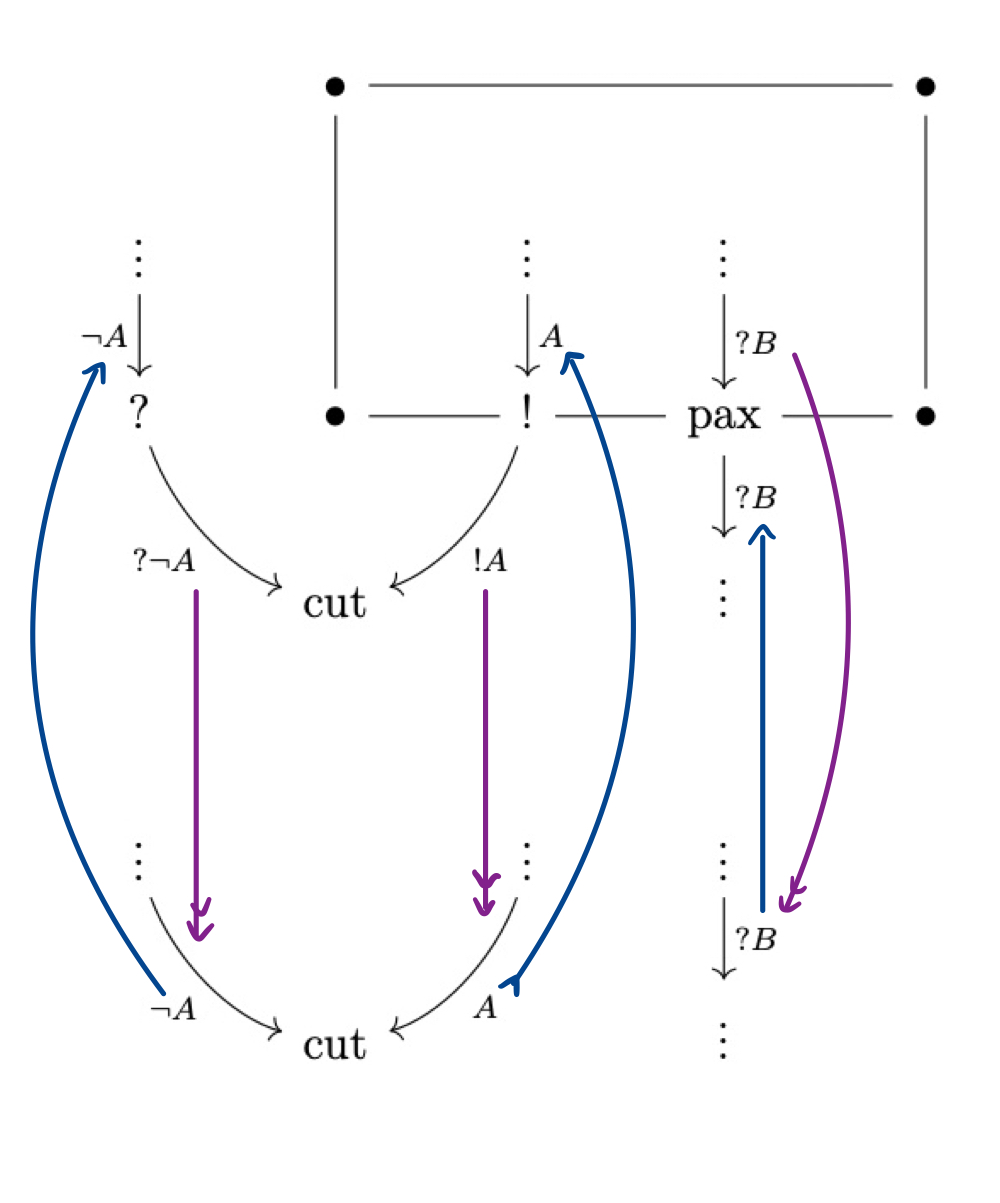
\includegraphics[width=0.5\textwidth]{DerTS.jpeg}
\caption{$!/?$-reduction where $TS \neq \operatorname{id}$}
\end{figure}

\begin{figure}[h]\label{fig:PaxST}
\centering
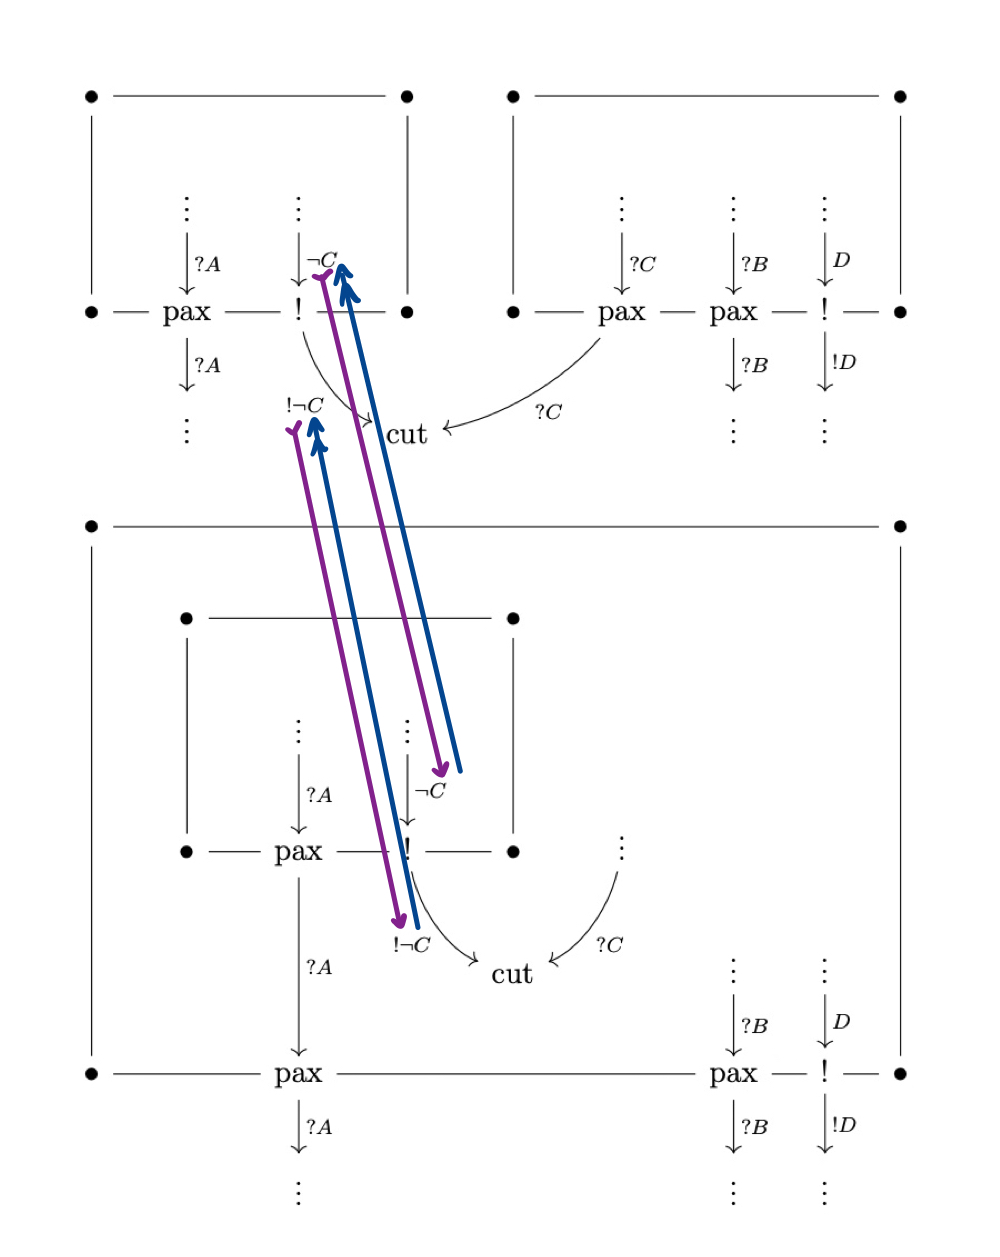
\includegraphics[width=0.5\textwidth]{PaxST.jpeg}
\caption{$!/\pax$-reduction where $ST \neq \operatorname{id}$}
\end{figure}

\begin{figure}[h]\label{fig:CtrST}
\centering
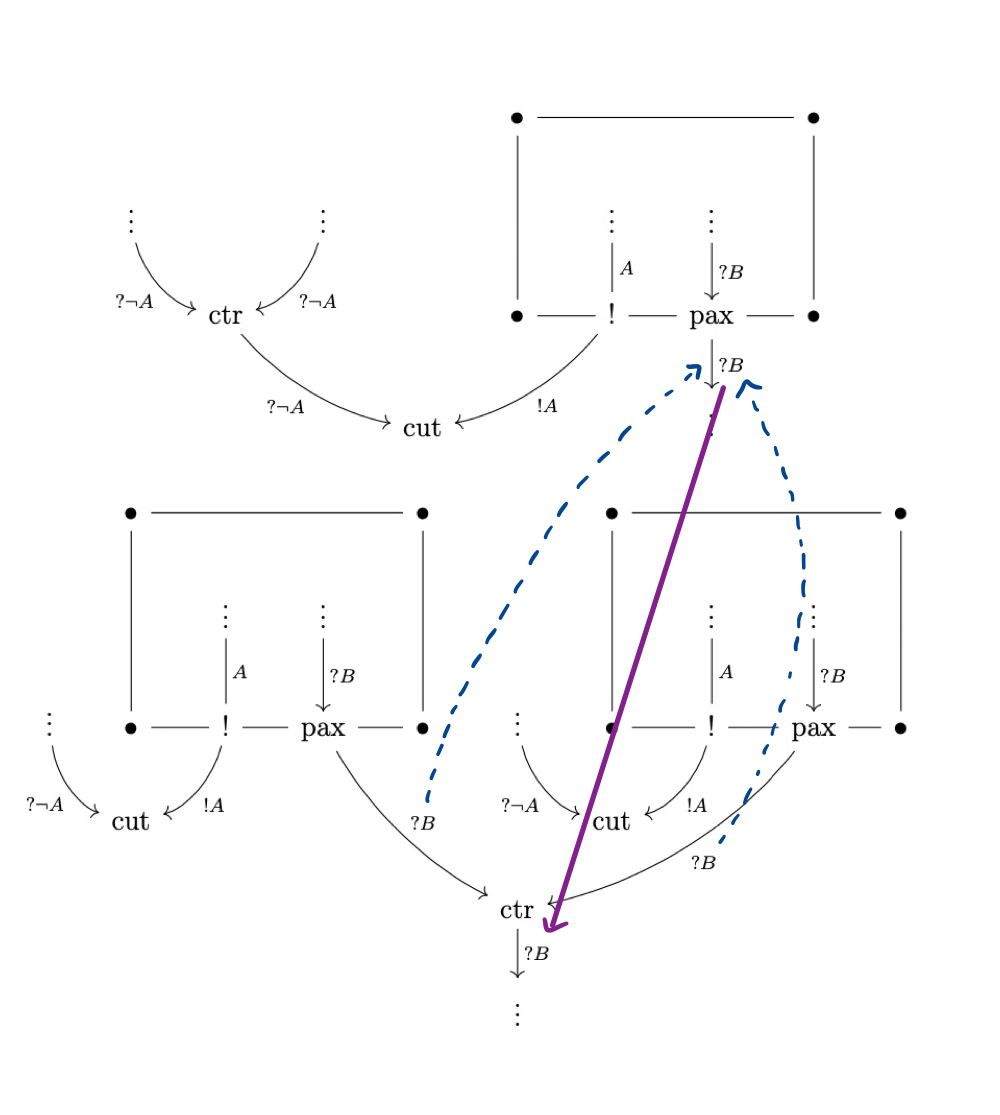
\includegraphics[width=0.5\textwidth]{CtrST.jpeg}
\caption{$!/\ctr$-reduction where $ST \neq \operatorname{id}$}
\end{figure}

\begin{figure}[h]\label{fig:CtrTS}
\centering
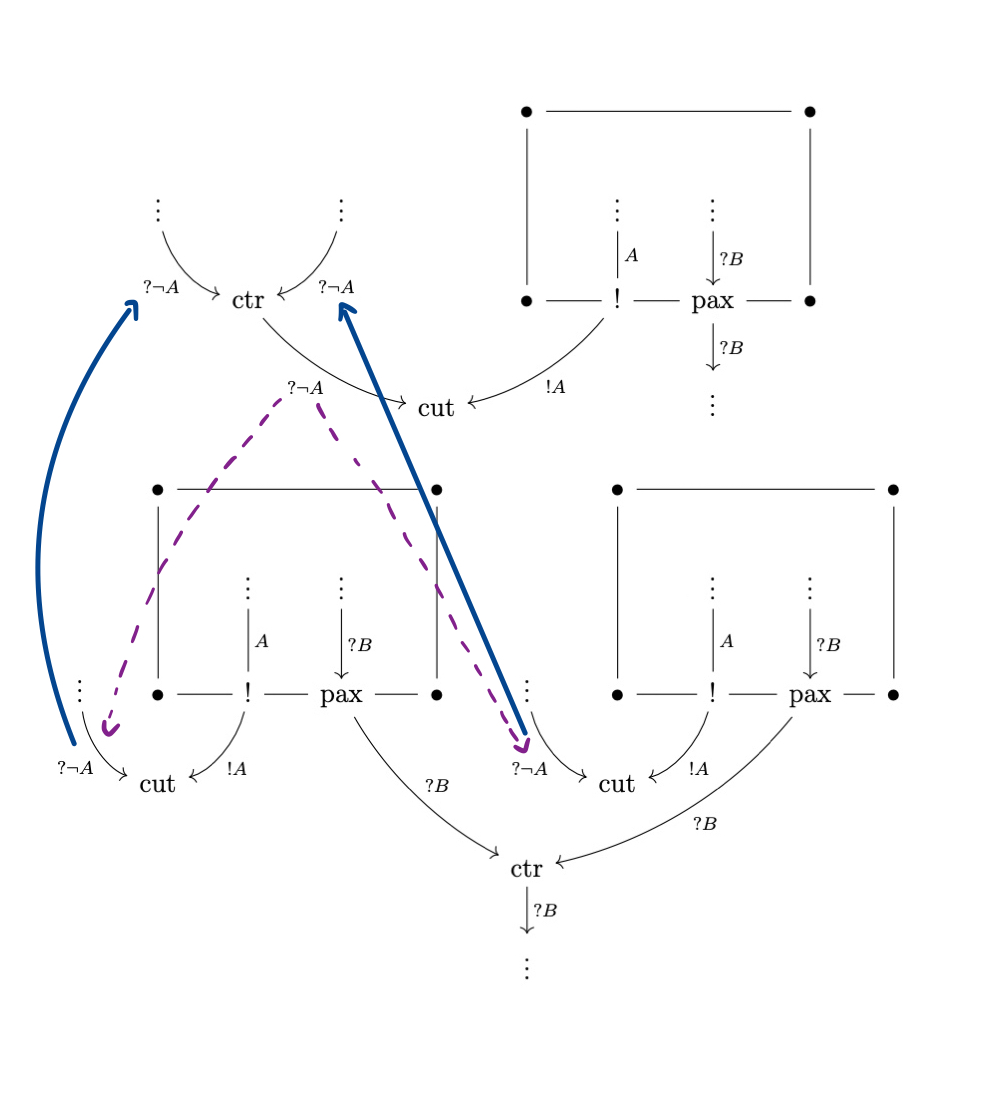
\includegraphics[width=0.5\textwidth]{CtrTS.jpeg}
\caption{$!/\ctr$-reduction where $TS \neq \operatorname{id}$}
\end{figure}

The most difficult case is when $\gamma$ reduces a $p$-redex and we have to show $p(S_\gamma T_\gamma - 1) = 0$. We only prove the case where all axiom links have atomic conclusions. By considering obvious extensions of $T_\gamma, S_\gamma$ to the $\eta$-expansion rules, the general case reduces to this case. We reference Diagram \eqref{eq:p_redex}. If $\textbf{X}$ is an unoriented atom of any of the displayed formulas other than $\neg C, !\neg C$, then the result is simple. Also, since $\operatorname{Dep}U_{\neg C} = \operatorname{Dep}U_{!\neg C}$ and each element of one of these sets is equated to the corresponding element in the other in the quotient ring $R_\pi$ it suffices to prove the result in the case where $\textbf{X} \in \operatorname{Dep}U_{\neg C}$.

We have $ST(j_1, j_2, \textbf{X}) = (0, j_2, \textbf{X}) \neq (j_1, j_2, \textbf{X})$ if $j_1 \neq 0$. By Lemma \ref{lem:global_equivalence} if $T(j_1, j_2, \textbf{X}) = (j_2, \textbf{X}) \not\sim 0$ then there exists some premise $E_{j_2}$ of the boxes of $\pi$ involved in the $p$-redex and $\textbf{X}'_{j_2}$ a variable of $\operatorname{Dep}U_{E_{j_2}}$ such that $\textbf{X} \sim \textbf{X}'_{j_2}$. By the definition of the equivalence relation, $T\big((j_2, \textbf{X})\big) - \textbf{X}'_{j_2} \in I_\pi$. Thus, this polynomial can be written as a linear combination
\begin{equation}
	\alpha_1 q_1 + \ldots + \alpha_t q_t = (j_2, \textbf{X}) - \textbf{X}'_{j_2}
\end{equation}
where $\alpha_1, \ldots, \alpha_t \in P_\pi$ and $q_1, \ldots, q_r$ are generators of $I_\pi$.

By applying $S$ to this linear combination we obtain
\begin{equation}
	S(\alpha_1) S(q_1) + \ldots + S(\alpha_t) S(q_t) = S(j_2, \textbf{X}) - S(\textbf{X}'_{j_2})
\end{equation}
where $S(q_1), \ldots, S(q_t) \in I_{\pi'}$ by the first part of this proof (where we showed $S(I_\pi) \subseteq I_{\pi'}$).

There are two cases, first say $\mathbf{X} \in \operatorname{Dep}U_{B_k}$ for some $1 \leq k \leq m$. Then $S(\mathbf{X'}_{j_2}) = \mathbf{X'}_{j_2}$ and $ST\big((j_1, j_2, \mathbf{X})\big) = (0, j_2, \mathbf{X}) \sim \mathbf{X'}_{j_2}$. By replacing all instances of $(0, j_2, \textbf{Y})$ among the $S(q_1), \ldots, S(q_t)$ by $(j_1, j_2, \textbf{Y})$ we see also that $(j_1, j_2, \textbf{X}) \sim \textbf{X}_{j_2}$, where the crucial observation is that $\textbf{X}_{j_2}$ is independent of $j_1$. Thus $(j_1, j_2, \textbf{X}) \sim (0, j_2, \textbf{X}) = ST(j_1, j_2, \textbf{X})$ and we are done.

Now say $\mathbf{X} \in \operatorname{Dep}U_{A_k}$ for some $1 \leq k \leq m$, the argument is very similar to the previous case but with one extra step. We obtain $(j_3, \textbf{X}'_{j_2}) \in \operatorname{Dep}U_{?A_k}$ in $P_\pi$ such that $(j_3, \textbf{X}'_{j_2}) \sim T(j_1, j_2, \textbf{X}) = (j_2, \textbf{X})$ as before, but we make the further observation that $(j_3, \textbf{X}'_{j_2}) \sim \textbf{X}'_{j_2}$ and so although it seems $(j_3, \textbf{X}'_{j_2})$ depends on $j_3$, it in fact does not. We thus assume $j_3 = 0$. We thus have
\begin{equation}
	ST(j_1, j_2, \textbf{X}) = (0, j_2, \textbf{X}) \sim S(0, \textbf{X}'_{j_2}) = (0,0, \textbf{X}'_{j_2})
\end{equation}
Making a similar substitution to the polynomials witnessing this equivalence shows $(j_1, j_2, \textbf{X}) \sim (0, 0, \textbf{X}'_{j_2}) \sim ST(j_1, j_2, \textbf{X})$ for all $j_1, j_2 \geq 0$, and we are done.

The remaining cases follow similarly to \cite[Proposition 4.6]{AlgPnt}.
\end{proof}

\begin{cor}
Let $\gamma: \pi \lto \pi'$ be a reduction of proof structures. Then $I_{\pi'} = T_\gamma^{-1}(I_\pi)$ or, identifying $P_{\pi'}$ as a subring of $P_\pi$ with inclusion $T_\gamma$,
\begin{equation}
I_{\pi'} = I_\pi \cap P_{\pi'}
\end{equation}
\end{cor}
\begin{proof}
Identical to that of \cite[Corollary 4.7]{MT}.
\end{proof}

\begin{remark}
There is the following proof structure whose cut link can \emph{not} be eliminated.
% https://q.uiver.app/?q=WzAsMTQsWzIsMSwiXFxvcGVyYXRvcm5hbWV7YXh9Il0sWzEsMiwiXFxuZWcgQSJdLFszLDIsIkEiXSxbMSwzLCI/Il0sWzMsNSwiISJdLFsxLDYsIj9cXG5lZyBBIl0sWzMsNiwiIUEiXSxbMiw3LCJcXG9wZXJhdG9ybmFtZXtjdXR9Il0sWzQsNSwiXFxidWxsZXQiXSxbNCwwLCJcXGJ1bGxldCJdLFswLDAsIlxcYnVsbGV0Il0sWzAsNSwiXFxidWxsZXQiXSxbMSw1LCJcXG9wZXJhdG9ybmFtZXtwYXh9Il0sWzEsNCwiP1xcbmVnIEEiXSxbMCwxLCIiLDAseyJjdXJ2ZSI6Miwic3R5bGUiOnsiaGVhZCI6eyJuYW1lIjoibm9uZSJ9fX1dLFswLDIsIiIsMix7ImN1cnZlIjotMiwic3R5bGUiOnsiaGVhZCI6eyJuYW1lIjoibm9uZSJ9fX1dLFsyLDRdLFs0LDYsIiIsMix7InN0eWxlIjp7ImhlYWQiOnsibmFtZSI6Im5vbmUifX19XSxbNiw3LCIiLDIseyJjdXJ2ZSI6LTJ9XSxbNSw3LCIiLDAseyJjdXJ2ZSI6Mn1dLFsxMywxMl0sWzMsMTMsIiIsMCx7InN0eWxlIjp7ImhlYWQiOnsibmFtZSI6Im5vbmUifX19XSxbMSwzLCIiLDAseyJzdHlsZSI6eyJoZWFkIjp7Im5hbWUiOiJub25lIn19fV0sWzEyLDUsIiIsMCx7InN0eWxlIjp7ImhlYWQiOnsibmFtZSI6Im5vbmUifX19XSxbMTEsMTIsIiIsMCx7InN0eWxlIjp7ImhlYWQiOnsibmFtZSI6Im5vbmUifX19XSxbMTIsNCwiIiwwLHsic3R5bGUiOnsiaGVhZCI6eyJuYW1lIjoibm9uZSJ9fX1dLFs0LDgsIiIsMCx7InN0eWxlIjp7ImhlYWQiOnsibmFtZSI6Im5vbmUifX19XSxbOCw5LCIiLDAseyJzdHlsZSI6eyJoZWFkIjp7Im5hbWUiOiJub25lIn19fV0sWzksMTAsIiIsMCx7InN0eWxlIjp7ImhlYWQiOnsibmFtZSI6Im5vbmUifX19XSxbMTAsMTEsIiIsMCx7InN0eWxlIjp7ImhlYWQiOnsibmFtZSI6Im5vbmUifX19XV0=
\[\begin{tikzcd}
	\bullet &&&& \bullet \\
	&& {\operatorname{ax}} \\
	& {\neg A} && A \\
	& {?} \\
	& {?\neg A} \\
	\bullet & {\operatorname{pax}} && {!} & \bullet \\
	& {?\neg A} && {!A} \\
	&& {\operatorname{cut}}
	\arrow[curve={height=12pt}, no head, from=2-3, to=3-2]
	\arrow[curve={height=-12pt}, no head, from=2-3, to=3-4]
	\arrow[from=3-4, to=6-4]
	\arrow[no head, from=6-4, to=7-4]
	\arrow[curve={height=-12pt}, from=7-4, to=8-3]
	\arrow[curve={height=12pt}, from=7-2, to=8-3]
	\arrow[from=5-2, to=6-2]
	\arrow[no head, from=4-2, to=5-2]
	\arrow[no head, from=3-2, to=4-2]
	\arrow[no head, from=6-2, to=7-2]
	\arrow[line width=0.5mm, no head, from=6-1, to=6-2]
	\arrow[line width=0.5mm, no head, from=6-2, to=6-4]
	\arrow[line width=0.5mm, no head, from=6-4, to=6-5]
	\arrow[line width=0.5mm, no head, from=6-5, to=1-5]
	\arrow[line width=0.5mm, no head, from=1-5, to=1-1]
	\arrow[line width=0.5mm, no head, from=1-1, to=6-1]
\end{tikzcd}\]
This cannot be reduced as there is no reduction rule pertaining to this situation.

This was already the case in the multiplicative fragment though, forget not the following irreducible multiplicative proof structure.
% https://q.uiver.app/?q=WzAsNCxbMSwwLCJcXG9wZXJhdG9ybmFtZXtheH0iXSxbMCwxLCJcXG5lZyBBIl0sWzIsMSwiQSJdLFsxLDIsIlxcb3BlcmF0b3JuYW1le2N1dH0iXSxbMCwxLCIiLDAseyJjdXJ2ZSI6Miwic3R5bGUiOnsiaGVhZCI6eyJuYW1lIjoibm9uZSJ9fX1dLFswLDIsIiIsMix7ImN1cnZlIjotMiwic3R5bGUiOnsiaGVhZCI6eyJuYW1lIjoibm9uZSJ9fX1dLFsxLDMsIiIsMCx7ImN1cnZlIjoyfV0sWzIsMywiIiwyLHsiY3VydmUiOi0yfV1d
\[\begin{tikzcd}
	& {\operatorname{ax}} \\
	{\neg A} && A \\
	& {\operatorname{cut}}
	\arrow[curve={height=12pt}, no head, from=1-2, to=2-1]
	\arrow[curve={height=-12pt}, no head, from=1-2, to=2-3]
	\arrow[curve={height=12pt}, from=2-1, to=3-2]
	\arrow[curve={height=-12pt}, from=2-3, to=3-2]
\end{tikzcd}\]
\end{remark}

We now extend \cite[Proposition 4.11]{AlgPnt}. In this paper we have so far only considered the unoriented atoms of a formula, however the \emph{oriented} atoms are easily defined, one just remembers the orientation of the atom.

\begin{proposition}\label{prop:zero}
Let $\pi$ be a proof net with single conclusion $A$, and let
\begin{equation}
(Z_i, z_i)_{i \geq 0}
\end{equation}
be the sequence of oriented atoms of $A$. Let $\mathbf{U} := (U_{i_j}, u_{i_j})_{j \geq 0}$ be the subsequence consisting of the positive atoms, and $\mathbf{V} := (V_{i_k}, v_{i_k})_{k \geq 0}$ the sequence of negative atoms.
\begin{itemize}
	\item The inclusions $k[\mathbf{U}] \lto P_\pi$ and $k[\mathbf{V}] \lto P_\pi$ followed by the quotient $P_\pi \lto R_\pi$ are surjective $\beta_+, \beta_-$:
	\begin{equation}
		\begin{tikzcd}
		k[\mathbf{U}]\arrow[dr,"\beta_+"]\arrow[d]\\
		P_\pi\arrow[r,twoheadrightarrow] & R_\pi\\
		k[\mathbf{V}]\arrow[u]\arrow[ru, swap, "\beta_-"]
		\end{tikzcd}
	\end{equation}
	\item Formally inverting $\beta_-^{-1}$ as a relation and composing yields a relation $\beta_-^{-1}\beta_+: k[\mathbf{U}] \lto k[\mathbf{V}]$.
\end{itemize}
\end{proposition}

The equivalence classes of atoms of $A$ in $R_\pi$ are the generalisation of persistent paths. Note, these are not paths, as there may be (infinite) forks.

\begin{example}\label{ex:non_bijective}
	We note that in general the above maps $\beta_+, \beta_-$ are \emph{not} isomorphisms, even in the weakening free case, as is the case in the following proof net (which admits only a single persistent path).
% https://q.uiver.app/#q=WzAsNCxbMCwwLCJcXG9wZXJhdG9ybmFtZXt9QXgiXSxbMSwxLCI/Il0sWzAsMiwiXFxwYXJyIl0sWzAsMywiXFxvcGVyYXRvcm5hbWV7Y30iXSxbMiwzLCJcXG5lZyBYIFxccGFyciA/WCJdLFswLDIsIlxcbmVnIFgiLDIseyJjdXJ2ZSI6M31dLFswLDEsIlgiLDAseyJjdXJ2ZSI6LTJ9XSxbMSwyLCI/IFgiLDAseyJjdXJ2ZSI6LTJ9XV0=
\[\begin{tikzcd}
	{\operatorname{}Ax} \\
	& {?} \\
	\parr \\
	{\operatorname{c}}
	\arrow["{\neg X \parr ?X}", from=3-1, to=4-1]
	\arrow["{\neg X}"', curve={height=18pt}, from=1-1, to=3-1]
	\arrow["X", curve={height=-12pt}, from=1-1, to=2-2]
	\arrow["{? X}", curve={height=-12pt}, from=2-2, to=3-1]
\end{tikzcd}\]
\end{example}
\begin{example}\label{ex:ryvers}
The ``persistent paths'' needs not be paths, in fact they need not even be trees, as in the following example.
% https://q.uiver.app/#q=WzAsMTAsWzIsMSwiXFxvcGVyYXRvcm5hbWV7QXh9Il0sWzEsMiwiPyJdLFszLDMsIiEiXSxbMSwzLCJcXG9wZXJhdG9ybmFtZXtwYXh9Il0sWzAsMywiXFxidWxsZXQiXSxbMCwwLCJcXGJ1bGxldCJdLFs0LDAsIlxcYnVsbGV0Il0sWzQsMywiXFxidWxsZXQiXSxbMiw0LCJcXHBhcnIiXSxbMiw1LCJcXG9wZXJhdG9ybmFtZXtjfSJdLFswLDEsIlxcbmVnIFgiLDIseyJjdXJ2ZSI6Mn1dLFsxLDMsIj8gXFxuZWcgWCIsMl0sWzAsMiwiWCIsMCx7ImN1cnZlIjotMn1dLFsyLDMsIiIsMCx7InN0eWxlIjp7ImhlYWQiOnsibmFtZSI6Im5vbmUifX19XSxbMyw0LCIiLDAseyJzdHlsZSI6eyJoZWFkIjp7Im5hbWUiOiJub25lIn19fV0sWzQsNSwiIiwwLHsic3R5bGUiOnsiaGVhZCI6eyJuYW1lIjoibm9uZSJ9fX1dLFs1LDYsIiIsMCx7InN0eWxlIjp7ImhlYWQiOnsibmFtZSI6Im5vbmUifX19XSxbNiw3LCIiLDAseyJzdHlsZSI6eyJoZWFkIjp7Im5hbWUiOiJub25lIn19fV0sWzcsMiwiIiwwLHsic3R5bGUiOnsiaGVhZCI6eyJuYW1lIjoibm9uZSJ9fX1dLFszLDgsIj9cXG5lZyBYIiwyLHsiY3VydmUiOjJ9XSxbMiw4LCIhWCIsMCx7ImN1cnZlIjotMn1dLFs4LDksIj9cXG5lZyBYIFxccGFyciAhWCJdXQ==
\[\begin{tikzcd}
	\bullet &&&& \bullet \\
	&& {\operatorname{Ax}} \\
	& {?} \\
	\bullet & {\operatorname{pax}} && {!} & \bullet \\
	&& \parr \\
	&& {\operatorname{c}}
	\arrow["{\neg X}"', curve={height=12pt}, from=2-3, to=3-2]
	\arrow["{? \neg X}"', from=3-2, to=4-2]
	\arrow["X", curve={height=-12pt}, from=2-3, to=4-4]
	\arrow[no head, from=4-4, to=4-2]
	\arrow[no head, from=4-2, to=4-1]
	\arrow[no head, from=4-1, to=1-1]
	\arrow[no head, from=1-1, to=1-5]
	\arrow[no head, from=1-5, to=4-5]
	\arrow[no head, from=4-5, to=4-4]
	\arrow["{?\neg X}"', curve={height=12pt}, from=4-2, to=5-3]
	\arrow["{!X}", curve={height=-12pt}, from=4-4, to=5-3]
	\arrow["{?\neg X \parr !X}", from=5-3, to=6-3]
\end{tikzcd}\]
\end{example}

\section{Geometry of Interaction One, Exponentials}
We take a moment to recall Geometry of Interaction One for multiplicative proof nets. Let $\pi$ be such a proof and assume $\pi$ has a single conclusion $A$. Then we have a special case of Proposition \ref{prop:zero} where $\beta_+, \beta_-$ are isomorphisms and the relation $\beta_-^{-1}\beta_+$ induces a permutation $\sigma$ on the unoriented atoms $U_A$ of $A$.

If we assume further that $\pi$ is $\cut$-free, and write the permutation $\sigma$ as a matrix with incdices labelled by $U_A$ then we obtain Girard's interpretation $\llbracket \pi \rrbracket$ of $\pi$ as given in \cite{girard}.

This generalises immediately to the case of exponentials where we simply allow for infinite dimensional matrices. The matrix corresponding to Example \ref{ex:non_bijective} is:
\begin{equation}\label{eq:ill}
	\llbracket \pi \rrbracket =
	\kbordermatrix{
		& X & (0, X) & (1, X) & (2, X) & \ldots\\
		X & 0 & 1 & 1 & 1 & \ldots\\
		(0,X) & 1  & 0 & 0 & 0 & \ldots\\
		(1,X) & 1 & 0 & 0 & 0 & \ldots\\
		(2,X) & 1 & 0 & 0 & 0 & \ldots\\
		\vdots & \vdots & \vdots & \vdots & \vdots & \ddots}
\end{equation}

The matrix corresponding to Example \ref{ex:ryvers} is given as follows.
\begin{equation}
	\kbordermatrix{
	& (0, X) & (0, X') & (1, X) & (1, X') & (2, X) & (2, X') & \ldots\\
	(0, X) & 0 & 1 & 0 & 0 & 0 & 0 & \ldots\\
	(0, X') & 1 & 0 & 0 & 0 & 0 & 0 & \ldots\\
	(1, X) & 0 & 0 & 0 & 1 & 0 & 0 & \ldots\\
	(1, X') & 0 & 0 & 1 & 0 & 0 & 0 & \ldots\\
	(2, X) & 0 & 0 & 0 & 0 & 0 & 1 & \ldots\\
	(2, X') & 0 & 0 & 0 & 0 & 1 & 0 & \ldots\\
	\vdots & \vdots & \vdots & \vdots & \vdots & \vdots & \vdots & \ddots
	}
	=
	\begin{bmatrix}
		J & 0 & \ldots\\
		0 & J & \ldots\\
		\vdots & \vdots & \ddots
	\end{bmatrix}
\end{equation}
where $J$ is the $2 \times 2$ matrix with $1$'s on the off diagraonal.

Returning to the multiplicative case, if $U_A$ has $n$ elements (recall $U_A$ is necessarily finite as we have assumed that $\pi$ is multiplicative) then the matrix $\llbracket \pi \rrbracket$ is to be read as a linear transformation:
\begin{equation}
	\llbracket \pi \rrbracket: (\ell^2)^{\oplus n} \lto (\ell^2)^{\oplus n}
\end{equation}
This situation does \emph{not} immediately generalise to the exponential setting because the matrices arrising may give ill-defined linear transformations. For instance, \eqref{eq:ill} is \emph{not} a valid linear transformation $\bigoplus_{U_{\neg X \parr ? X}}\ell^2 \lto \bigoplus_{U_{\neg X \parr ? X}}\ell^2$ as there exists a column with infinitely many 1's.

\section{The equivariant Buchberger algorithm}

Let $k$ be a field and denote by $\call{V}$ a countably infinite set of variables $\call{V} = \{ x_0, x_1, \ldots \}$. Denote by $R$ the ring of polynomials over these variables $R = k[\call{V}]$ with coefficients in $k$. We denote by $\Pi$ the monoid of increasing functions $f: \bb{N} \lto \bb{N}$ (with multiplication given by composition and unit given by the identity function). There exists an action of $\Pi$ on $\call{V}$ given as follows, for a function $\rho \in \Pi$ and $i \in \bb{N}$ we have $\rho \cdot x_i = x_{\rho(i)}$. We algebraically extend this to an action of $\Pi$ on $R$ as follows
\begin{equation}
	\rho\cdot(\alpha p) := \alpha \rho\cdot p,\quad \rho\cdot(p + q) := \rho\cdot p + \rho \cdot q,\quad \rho\cdot(pq) := (\rho\cdot p)(\rho\cdot q)
\end{equation}
Thus, $R$ has the structure of both an $R$-algebra and also a $\Pi$-action. We can capture both of these actions by extending the scalars of $R$.
\begin{defn}
	Let $R \ast \Pi$ denote the ring whose underlying set consists of formal sums
	\begin{equation}
		\sum_{\rho \in \Pi}f_\rho \cdot \rho
	\end{equation}
	where $\{f_\rho\}_{\rho \in \Pi}$ is a finite subset of $R$.

	Given $f,g \in R$ and $\rho, \sigma \in \Pi$ we define the multiplication of $f\rho, g\sigma$ as follows:
	\begin{equation}
		(f\cdot \rho)(g\cdot \sigma) := f\rho(g)\cdot\rho\sigma
	\end{equation}
	where $f\rho(g)$ is the result of multiplying $f$ and $\rho(g)$ in $R$, and $\rho\sigma$ is the result of multiplying $\rho$ and $\sigma$ in $\Pi$.
\end{defn}

The ring $R$ is an $R \ast \Pi$-algebra. To see this, notice first that since $\Pi$ act on $R$ and $R$ is a ring, that multiplication by any $\rho \in \Pi$ is a ring homomorphism $R \lto R$. Thus:
\begin{align*}
	\big((f\cdot \rho)(g \cdot \sigma)\big)h &= \big((f \rho(g))\cdot \rho \sigma\big)h\\
	&= f\rho(g)(\rho\sigma\cdot h)
\end{align*}
and on the other hand,
\begin{align*}
	(f\cdot \rho)\big((g \cdot \sigma ) h\big) &= (f \cdot \rho)(g \sigma \cdot h)\\
	&= (f \rho\big(g \sigma \cdot h\big))\\
	&= f \rho (g) (\rho\sigma) \cdot h
\end{align*}
So $R$ can equivalently be thought of as a $R \ast \Pi$-algebra. \textcolor{red}{Do we get the distributivity laws? I don't think I've checked these.}

We will denote by $M$ the ideal generated by $\call{V}$ in $R$.

\begin{defn}
	Let $F$ be a subset of $R$. We denote by $\langle F \rangle_\Pi$ the ideal generated by $F$ and the action of $\Pi$ on $R$. That is,
	\begin{equation}
		\langle F \rangle_\Pi := \{ h \rho f \mid h \in R, \rho \in \Pi, f\in F \}
	\end{equation}
\end{defn}

If we let $\langle F \rangle$ denote the ideal generated by $F$ in $R$ as an $R \ast \Pi$-algebra then $\langle F \rangle = \langle F \rangle_\Pi$.

\begin{defn}
	An ideal $I \subseteq R$ is \textbf{$\Pi$-finitely generated} if there exists a finite subset $F \subseteq I$ such that
	\begin{equation}
		I = \langle F \rangle_\Pi
	\end{equation}
\end{defn}

\begin{lemma}
	All ideals of $R$ are $\Pi$-finitely generated. In other words, $R$ is a Noetherian $R\ast \Pi$-module.
\end{lemma}
\begin{proof}
\textcolor{red}{Proof needed.}
\end{proof}

\begin{defn}
A \textbf{monomial ordering} $>$ on $R$ is a relation $>$ on $\bb{Z}_{\geq 0}^n$, or equivalently, a relation on the set of monomials $x^\alpha, \alpha \in \bb{Z}_{\geq 0}^n$, satisfying:
\begin{itemize}
	\item $>$ is a total ordering on $\bb{Z}_{\geq 0}^n$.
	\item If $\alpha > \beta$ and $\gamma \in \bb{Z}_{\geq 0}^n$, then $\alpha + \gamma > \beta + \gamma$.
	\item $>$ is a well-ordering on $\bb{Z}_{\geq 0}^n$. That is, every non-empty subset of $\bb{Z}_{\geq 0}^n$ has a least element under $>$.
\end{itemize}
\end{defn}

We will denote by $M$ the ideal of monomials of $R$. That is, $M = \langle \call{V} \rangle$.

\begin{lemma}\label{lem:lexico_monomial}
	If we arbitrarily order $\call{V}$: $x_0 < x_1 < \ldots$ then lexicographic order on $M$ induced by this order is a monomial order.
\end{lemma}
\begin{proof}
\textcolor{red}{Proof needed. Also, is this $\Pi$-respecting?}.
\end{proof}

\begin{algorithm}\label{alg:division}
	\caption{Equivariant Euclidean Division with Early Stopping}\label{alg:division_adapted}
	\begin{algorithmic}
		\Require $(f_1,\ldots,f_n),f$
		\State $p \gets f$
		\State $q_1,\ldots, q_n \gets 0,\ldots 0$
		\State $\rho_1, \ldots, \rho_n \gets e, \ldots, e$
		\State $r \gets 0$
		\While{$p \neq 0$}
		\State $\text{DivOcc} \gets \texttt{False}$
		\State $i \gets 1$
		\While{$i \leq n \text{ and } \text{DivOcc} = \texttt{false}$}
		\If{$\exists \rho \in \Pi, \operatorname{LT}\rho f_i | \operatorname{LT}p$}
		\State $\text{Choose }\rho\in \Pi, \rho f_i \mid \operatorname{LT} p$
		\State $\rho_i \gets \rho$
		\State $q_i \gets q_i + \operatorname{LT}p/\operatorname{LT}\rho f_i$
		\State $p \gets p - (\operatorname{LT}p/\operatorname{LT}\rho f_i)\rho f_i$
		\State $\text{DivOcc} \gets \texttt{True}$
		\Else 
		\State $i \gets i + 1$
		\EndIf
		\EndWhile
		\If{$\operatorname{DivOcc} = \texttt{false}$}
		\State $r \gets p$
		\State $p \gets 0$
		\EndIf
		\EndWhile\\
		\Return{$(q_1,\ldots,q_n, \rho_1, \ldots, \rho_n, r)$}
	\end{algorithmic}
\end{algorithm}

\begin{remark}
In Algorithm \ref{alg:division} one of the steps is to choose $\rho \in |pi, \rho f_i \mid \operatorname{LT}p$. This may seem non-algorithmic but we satisfy ourselves with this pseudocode as the proof of Lemma \ref{lemma:lcm} implicitly describes a method for constructing a canonical choice of $\rho$.
\end{remark}

\begin{lemma}
Let $G = (f_1, \ldots, f_n)$ be a sequence of elements of $R$. Given $f \in R$ let $(q_1, \ldots, q_n, r)$ be the output of Algorithm \ref{alg:division}. Then
\begin{equation}\label{eq:division_result}
f = q_1 \rho_1 f_1 + \ldots + q_n \rho_n f_n + r
\end{equation}
and if $r \neq 0$ the leading term of $r$ is not $\Pi$-divisible by any $\operatorname{LT}f_i$ with $1 \leq i \leq s$. Furthermore, if $q_i f_i \neq 0$ then $\operatorname{multideg}f \geq \operatorname{multideg}(q_i f_i)$.
\end{lemma}
\begin{proof}
The expression $f = \sum_{i = 1}^n q_i \rho_i f_i + p + r$ holds at the end of every iteration of the outer while loop, and it terminates with $p = 0$, so the \eqref{eq:division_result}. \textcolor{red}{Rest of proof needed.}
\end{proof}




\begin{lemma}\label{lemma:lcm}
Consider two monomials in $R$:
\begin{equation}
m_1 = x_{i_1}^{k_1}\ldots x_{i_n}^{k_n},\quad m_2 = x_{j_1}^{l_1}\ldots x_{j_m}^{l_m}, \quad m \geq n
\end{equation}
Then the least common multiple of $m_1, m_2$ in $R$ as an $R \ast \Pi$-module is:
\begin{equation}
\label{eq:lcm}
x_{\operatorname{max}\{i_1, j_1\}}^{\operatorname{max}\{k_1, l_1\}}\cdots x_{\operatorname{max}\{i_n, j_n\}}^{\operatorname{max}\{k_n, l_n\}}x_{j_{n+1}}^{l_{n+1}}\cdots x_{k_m}^{l_m}
\end{equation}
\end{lemma}
\begin{proof}
Let $m$ denote the monomial of \eqref{eq:lcm}. There exists a non-decreasing function $\rho_1: \bb{N} \lto \bb{N}$ such that $\rho_1(i_1) = \operatorname{max}\{i_1, j_1\}, \ldots, \rho_1(i_n) = \operatorname{max}\{i_n, j_n \}$. The action of this map on $m_1$ is given as follows.
\begin{equation}
\rho_1(m_1) = x_{\operatorname{max}\{i_1, j_1\}}^{k_1}\ldots x_{\operatorname{max}\{i_n, j_n\}}^{k_n}
\end{equation}
Thus, $\rho_1(m_1) \mid m$ which implies $m_1 \mid_\Pi m$. Similarly, an increasing function $\rho_2: \bb{N} \lto \bb{N}$ can be constructed so that $\rho_2(m_2) \mid m$. Thus $m$ is a common multiple of $m_1, m_2$.

To show that it is the least such, say $m'$ was a monomial such that $m_1 \mid_\Pi m'$ and $m_2 \mid_\Pi m'$. Write $m' = x_{r_1}^{t_1}\ldots x_{r_s}^{t_s}$. Since $m_1 \mid_\Pi m'$ and $m_2 \mid_\Pi m'$ we have $s \geq m$. Also, the action of $\Pi$ on $R$ does not change the powers of any of the variables in a monomial, thus
\begin{equation}
t_1 \geq \operatorname{max}\{k_1, l_1\}, \ldots, t_n \geq \operatorname{max}\{k_n, l_n\}, t_{n+1} \geq l_{n+1}, \ldots, t_m \geq l_m
\end{equation}
Lastly, since $\Pi$ is contains only non-decreasing functions, it follows from $m_1 \mid_\Pi m'$ and $m_2 \mid_\Pi m'$ that
\begin{equation}
\operatorname{max}\{i_1, j_1\} \leq r_1, \ldots, \operatorname{max}\{i_n, j_n\} \leq r_n, j_{n+1} \leq r_{n+1}, \ldots, j_{m} \leq r_m
\end{equation}
Thus, $m \mid_\Pi m'$.
\end{proof}

In the setting of the standard Buchberger Algorithm, the \emph{$S$-polynomials} are used to determine whether a given generating set is a Gr\"{o}bner basis or not. We recall the definition of the $S$-polynomial.

\begin{defn}
Let $f, g \in k[x_1, \ldots, x_n]$. The \textbf{$S$-polynomial} $S(f,g)$ of $f,g$ is
\begin{equation}
S(f,g) := \frac{x^\gamma}{\operatorname{LT}f}f - \frac{x^\gamma}{\operatorname{LT}g}g
\end{equation}
where $x^\gamma = \operatorname{lcm}(\operatorname{LT}f, \operatorname{LT}g)$.
\end{defn}

In this setting, the pair $\big(x^\gamma/\operatorname{LT}f, x^\gamma/\operatorname{LT}g)\big)$ is the unique, minimal pair of monomials $(h,j)$ such that $\operatorname{hf} = \operatorname{LT}jg$, where minimality $\big(x^\gamma/\operatorname{LT}f, x^\gamma/\operatorname{LT}g)\big) \leq (h, j)$ means $x^\gamma/\operatorname{LT}f \mid h$ and $x^\gamma/\operatorname{LT}g \mid j$.

\begin{defn}
Let $f, g \in R = k[x_0, x_1, \ldots]$. The \textbf{$\Pi$-$S$-polynomial} $S(f,g)$ of $f, g$ is
\begin{equation}
S^\Pi(f,g) := \frac{x^\gamma}{\rho_1 \operatorname{LT}f}\rho_1 f - \frac{x^\gamma}{\rho_2 \operatorname{LT}g}\rho_2 g
\end{equation}
where $x^\gamma = \operatorname{lcm}(\operatorname{LT}f, \operatorname{LT}g)$ and $\rho_1, \rho_2$ are respectively elements of $\Pi$ such that $\rho_1 \operatorname{LT}f \mid x^\gamma$ and $\rho_2 \operatorname{LT}g \mid x^\gamma$, the existence of which was established in the proof of Lemma \ref{lemma:lcm}.
\end{defn}

\begin{defn}
Let $G = (f_1, \ldots, f_s)$ be a sequence of polynomials and $f$ a polynomial. We denote by $\operatorname{EqDiv}_{\text{es}}(f,G)$ the remainder $r$ produced by Equivariant Euclidean division (Algorithm \ref{alg:division}).
\end{defn}

There are only two significant differences between Algorithm \ref{alg:buchberger} and the standard Buchberger Algorithm (given for example in Theorem \cite[Theorem 9, \S 10]{Cox}). We use the Equivariant Euclidean Division Algorithm instead of the standard Euclidean Division Algorithm, and we add the entire $\Pi$-orbit $\operatorname{Orb}(f_t)$ of $f_t$ to $G$, rather than just $f_t$ itself.

\begin{algorithm}\label{alg:buchberger}
	\caption{Equivariant Buchberger with Early Stopping}\label{alg:elimination}
	\begin{algorithmic}
		\Require $F = (f_1,\ldots,f_s)$, returns a $\Pi$-equivariant Gröbner basis for $\langle f_1,\ldots,f_s \rangle_{\Pi}$.
		\State $B \gets \{ (i,j) \l 1 \le i < j \le s \}$
		\State $G \gets F$
		\State $t \gets s$
		\While{$B \neq \emptyset$}
		\State Let $(i,j) \in B$ be first in the lexicographic order.
		\If{$\operatorname{LCM}(\LM(f_i), \LM(f_j)) \neq \LM(f_i) \LM(f_j)$ \textbf{and} $\operatorname{Criterion}(f_i, f_j, B)$ \textbf{is false}}
		\State $S \gets \operatorname{EqDiv}_{\text{es}}{S(f_i, f_j)}{G}$
		\If{$S \neq 0$}
		\State $t \gets t + 1$
		\State $f_t \gets \frac{1}{\operatorname{LC}(S)}S$
		\State $G \gets G \cup \operatorname{Orb}(f_t)$
		\State $B \gets B \cup \{ (i,t) \l 1 \le i \le t - 1 \}$
		\EndIf
		\EndIf
		\State $B \gets B \setminus \{(i,j)\}$
		\EndWhile\\
	\Return{$G$}
	\end{algorithmic}
	where $\operatorname{Criterion}(f_i, f_j, B)$ is true provided that there is some $k \notin \{i,j\}$ for which the pairs $[i,k]$ and $[j,k]$ are \emph{not} in $B$ and $\LM(f_k)$ divides $\operatorname{LCM}(\LM(f_i),\LM(f_j))$.
\end{algorithm}

\section{Elimination Theory}
Elimination Theory begins with the following Theorem.
\begin{thm}
Let $G$ be a Gr\"{o}bner basis for an ideal $I \subseteq k[x_1, \ldots, x_n]$ with respect to the lexicographic monomial order induced by $x_1 < \ldots < x_n$. Then for any $l$ such that $1 \leq l \leq n-1$, the set
\begin{equation}
G \cap k[x_{l+1}, \ldots, x_n]
\end{equation}
is a Gr\"{o}bner basis for the ideal
\begin{equation}
I \cap k[x_{l+1}, \ldots, x_n]
\end{equation}
\end{thm}
\begin{proof}
See \cite[Chapter 3, \S 1, Theorem 2]{Cox}.
\end{proof}
We prove a generalisation of this Theorem to the setting where the polynomial ring is over infinitely many variables.
\begin{thm}
Let $G$ be a Gr\"{o}bner basis for an ideal $I \subseteq k[x_1, \ldots]$ with respect to the lexicographic monomial order induced by $x_1 < \ldots$. Then for any $l \geq 0$ the set
\begin{equation}
G \cap k[x_{l+1}, \ldots]
\end{equation}
is a Gr\"{o}bner basis for the ideal
\begin{equation}
I \cap k[x_{l+1}, \ldots]
\end{equation}
\end{thm}
\begin{proof}
Let $G_l$ denote the set $G \cap k[x_{l+1}, \ldots]$ and $I_l$ denote the ideal $I \cap k[x_{l+1}, \ldots]$. We must show
\begin{equation}
\langle \operatorname{LT}(I_l) \rangle = \langle \operatorname{LT}(G_l)\rangle
\end{equation}
We prove the non-obvious inclusion. Let $f \in I_l$ and consider $\operatorname{LT}f$. Since $I_l \subseteq I$ we have that $f \in I$. Moreover, $G$ is a G\"{o}bner basis for $I$ and so there exists $g \in G$ such that $\operatorname{LT}(g) \mid \operatorname{LT}(f)$. Since we are working with respect to lexicographic ordering, this in fact implies that $g \in I_l$.
\end{proof}


\bibliographystyle{amsalpha}
	\providecommand{\bysame}{\leavevmode\hbox to3em{\hrulefill}\thinspace}
	\providecommand{\href}[2]{#2}
	\begin{thebibliography}{99}
		\bibitem{linearlogic} \emph{Linear Logic}, J.Y. Girard. Theoretical Computer Science, Volume 50, Issue 1, Jan. 30, 1987.
		
		\bibitem{multiplicatives} \emph{Multiplicatives}, J.Y. Girard. Logic and Computer Science: New Trends and Applications. Rosenberg \& Sellier. pp. 11--34 (1987).
		
		\bibitem{girard} \emph{Geometry of Interaction: Interpretation of System F}, J.Y. Girard. Categories in Computer Science and Logic, pages 69 – 108, Providence, 1989.
		
		\bibitem{GoI2} \emph{Geometry of Interaction II, Deadlock Free Agorithms} Part of the Lecture Notes in Computer Science book series (LNCS,volume 417). 2005.
		
		\bibitem{GoI3} \emph{Geometry of Interaction III, Accomodation the Additives}, J.Y. Girard. Proceedings of the workshop on Advances in linear logic. June 1995
		
		\bibitem{GoI4} \emph{Geometry of Interaction IV, the Feedback Equation}, J.Y. Girard. Logic Colloquium 2003, December 9.
		
		\bibitem{GoI5} \emph{Geometry of Interaction V}, J.Y. Girard. Theoretical Computer ScienceVolume 412Issue 20April, 2011
		
		\bibitem{Regnier} \emph{Linear Logic and the Hilbert Space} Advances in Linear Logic , pp. 307 - 328, Cambridge University Press, 1995.
		
		\bibitem{Seiller1} \emph{Interaction Graphs: Multiplicatives} Annals of Pure and Applied Logic 163 (2012), pp. 1808-1837.
		
		\bibitem{Seiller2} \emph{Interaction Graphs: Additives} Annals of Pure and Applied Logic 167 (2016), pp. 95-154.
		
		\bibitem{Seiller3} \emph{Interaction Graphs: Nondeterministic Automata}, ACM Transactions in Computational Logic 19(3), 2018.
		
		\bibitem{Seiller4} \emph{Interaction Graphs: Exponentials} Logical Methods in Computer Science 15, 2019.
		
		\bibitem{Laurent} \emph{Olivier Laurent. A Token Machine for Full Geometry of Interaction}. 2001, pp.283-297. ⟨hal-00009137⟩
		
		\bibitem{HaghverdiScott} \emph{Towards a Typed Geometry of Interaction} CSL 2005: Computer Science Logic pp 216–231.
		
		\bibitem{Hines} \emph{From a conjecture of Collatz to Thompson's group F, via a conjunction of Girard}, \url{https://arxiv.org/abs/2202.04443}
		
		\bibitem{BS} \emph{The Blind Spot}. J.Y. Girard.
		
		\bibitem{AnalyticFunctors} \emph{Normal functors, power series and lambda-calculus} Annals of Pure and Applied Logic
		Volume 37, Issue 2, February 1988, Pages 129-177.
		
		\bibitem{GMZ} \emph{Gentzen-Mints-Zucker Duality} D. Murfet, W. Troiani. \url{https://arxiv.org/abs/2008.10131}
		
		\bibitem{laurent} \emph{An introduction to proof nets}. O. Laurent. \url{http://perso.ens-lyon.fr/olivier.laurent/pn.pdf}
		
		\bibitem{AlgPnt} \emph{Elimination and cut-elimination in multiplicative linear logic}, W. Troiani, D. Murfet.
		
		\bibitem{Frege} \emph{Sense and Reference} G. Frege. Philosophical Review 57 (3):209-230 (1948)
		
		\bibitem{Sorensen} \emph{Lectures on the Curry-Howard Isomorphism} Published: July 4, 2006 Imprint: Elsevier Science

		\bibitem{MT} \emph{Elimination and cut-elimination in multiplicative linear logic}

		\bibitem{Cox} Cox, Little, OShea
		
	\end{thebibliography}

\end{document}